\documentclass[a4paper,oneside,11pt]{book}

% Package dasar
\usepackage[utf8]{inputenc}     % untuk karakter UTF-8
\usepackage[T1]{fontenc}        % encoding font
\usepackage{graphicx}
\usepackage{titling}
\usepackage{titlesec}
\usepackage[backend=biber,style=ieee]{biblatex}
\addbibresource{ref.bib}

% Package tambahan untuk layout dan formatting
\usepackage{geometry}           % untuk margin
\usepackage{setspace}           % untuk spasi baris
\usepackage{fancyhdr}           % untuk header/footer
\usepackage{hyperref}           % untuk link dan bookmark
\usepackage{listings}           % untuk code Python
\usepackage{xcolor}             % untuk warna
\usepackage{float}              % untuk posisi gambar
\usepackage{tocloft}            % Untuk membuat daftar isi menampilkan "Bab 1. Pendahuluan" instead of "1. Pendahuluan",
\usepackage{lipsum}             % untuk lorem ipsum
\usepackage{indentfirst}        % untuk indent paragraf pertama

% Pengaturan layout
\geometry{left=3cm, right=2cm, top=2cm, bottom=2cm}
\onehalfspacing  % spasi 1.5

% Format chapter
\titleformat{\chapter}[hang]
  {\normalfont\huge\bfseries\centering}{\chaptertitlename\ \thechapter.}{1em}{}

% Format code Python
\lstset{
    language=PHP,
    basicstyle=\ttfamily\small,
    keywordstyle=\color{blue}\bfseries,
    commentstyle=\color{gray},
    stringstyle=\color{red},
    numbers=left,
    numberstyle=\tiny,
    frame=single,
    breaklines=true,
    showstringspaces=false,
    xleftmargin=2cm,
    xrightmargin=1cm,
    morekeywords={Route,Controller,Request,Response,Blade,Model,Migration,Artisan,middleware,Auth,extends,section,yield,csrf,foreach,endif}
}

% Pengaturan hyperref
\hypersetup{
    colorlinks=true,
    linkcolor=black,
    filecolor=magenta,
    urlcolor=blue,
    citecolor=red
}

% Info dokumen
\title{Dokumen \\ Proyek Aplikasi Dasar\\
UTS}
\author{Kelompok 21 (SIA WEB)\\
Anggota: \\
1. Nama 1 (123456789)\\
2. Nama 2 (123456789)\\
3. Nama 3 (123456789)\\
4. Nama 4 (123456789)}

\begin{document}

% Title Page
\begin{titlingpage} 
\begin{center}

\vspace{4cm} 
\begin{Large} 
\textbf{\thetitle} \\
\end{Large}
\vspace{2cm}


\includegraphics[height=8cm]{lambang ugm.png}\\ 
\begin{large}
\vspace{2cm} 
\theauthor\\ 
\end{large}

\vspace{2cm}
\begin{Large}
\textbf{Sekolah Vokasi}\\
\textbf{Universitas Gadjah Mada}\\
\textbf{Yogyakarta}\\
\textbf{2025}\\
\end{Large}

\end{center}
\end{titlingpage}

% Header/Footer
\pagestyle{fancy}
\fancyhf{}            % kosongkan header/footer default
\fancyfoot[C]{\thepage} % taruh nomor halaman di footer tengah


% --- Styling Judul Daftar Isi, Gambar, dan Kode ---
\renewcommand{\cfttoctitlefont}{\hfill\normalfont\LARGE\bfseries}
\renewcommand{\cftaftertoctitle}{\hfill}
\renewcommand{\cftbeforetoctitleskip}{1em}
\renewcommand{\cftaftertoctitleskip}{1.5em}

% --- Format Bab di Daftar Isi ---
\renewcommand{\cftchappresnum}{Bab~}
\renewcommand{\cftchapaftersnum}{.}
\renewcommand{\cftchapnumwidth}{3.5em}
\renewcommand{\cftchapfont}{\bfseries}
\renewcommand{\cftchappagefont}{\bfseries}

% --- Spasi dan Estetika ---
\setlength{\cftbeforechapskip}{0.8em} % jarak antar bab
\setlength{\cftbeforesecskip}{0.2em}  % jarak antar subbab
\renewcommand{\cftsecfont}{\normalfont}
\renewcommand{\cftsubsecfont}{\normalfont}

% --- Judul Lokal ---
\renewcommand{\contentsname}{\centering Daftar Isi}
\renewcommand{\listfigurename}{\centering Daftar Gambar}
\renewcommand{\lstlistlistingname}{\centering Daftar Kode}

% --- Gaya Daftar Gambar dan Daftar Kode ---
\renewcommand{\cftloftitlefont}{\hfill\normalfont\LARGE\bfseries}
\renewcommand{\cftafterloftitle}{\hfill}

\tableofcontents

\newpage
% Daftar Gambar
\listoffigures

\newpage


% Contoh gambar
% \begin{figure}[H]
%   \centering
%   \includegraphics[width=0.8\textwidth]{img/HasilTambah.png}
%   \caption{Hasil Tambah Simpanan}
%   \label{fig:hasil_tambah}
% \end{figure}

% Dokumen-Dokumen penting
\chapter{Dokumen}
\section{MVP}
\section{Bisreq}

\newpage
% Use Case
\section{Use Case}

% Subsystem manejer
\subsection{Subsystem: Manajerial}
\begin{figure}[H]
  \centering
  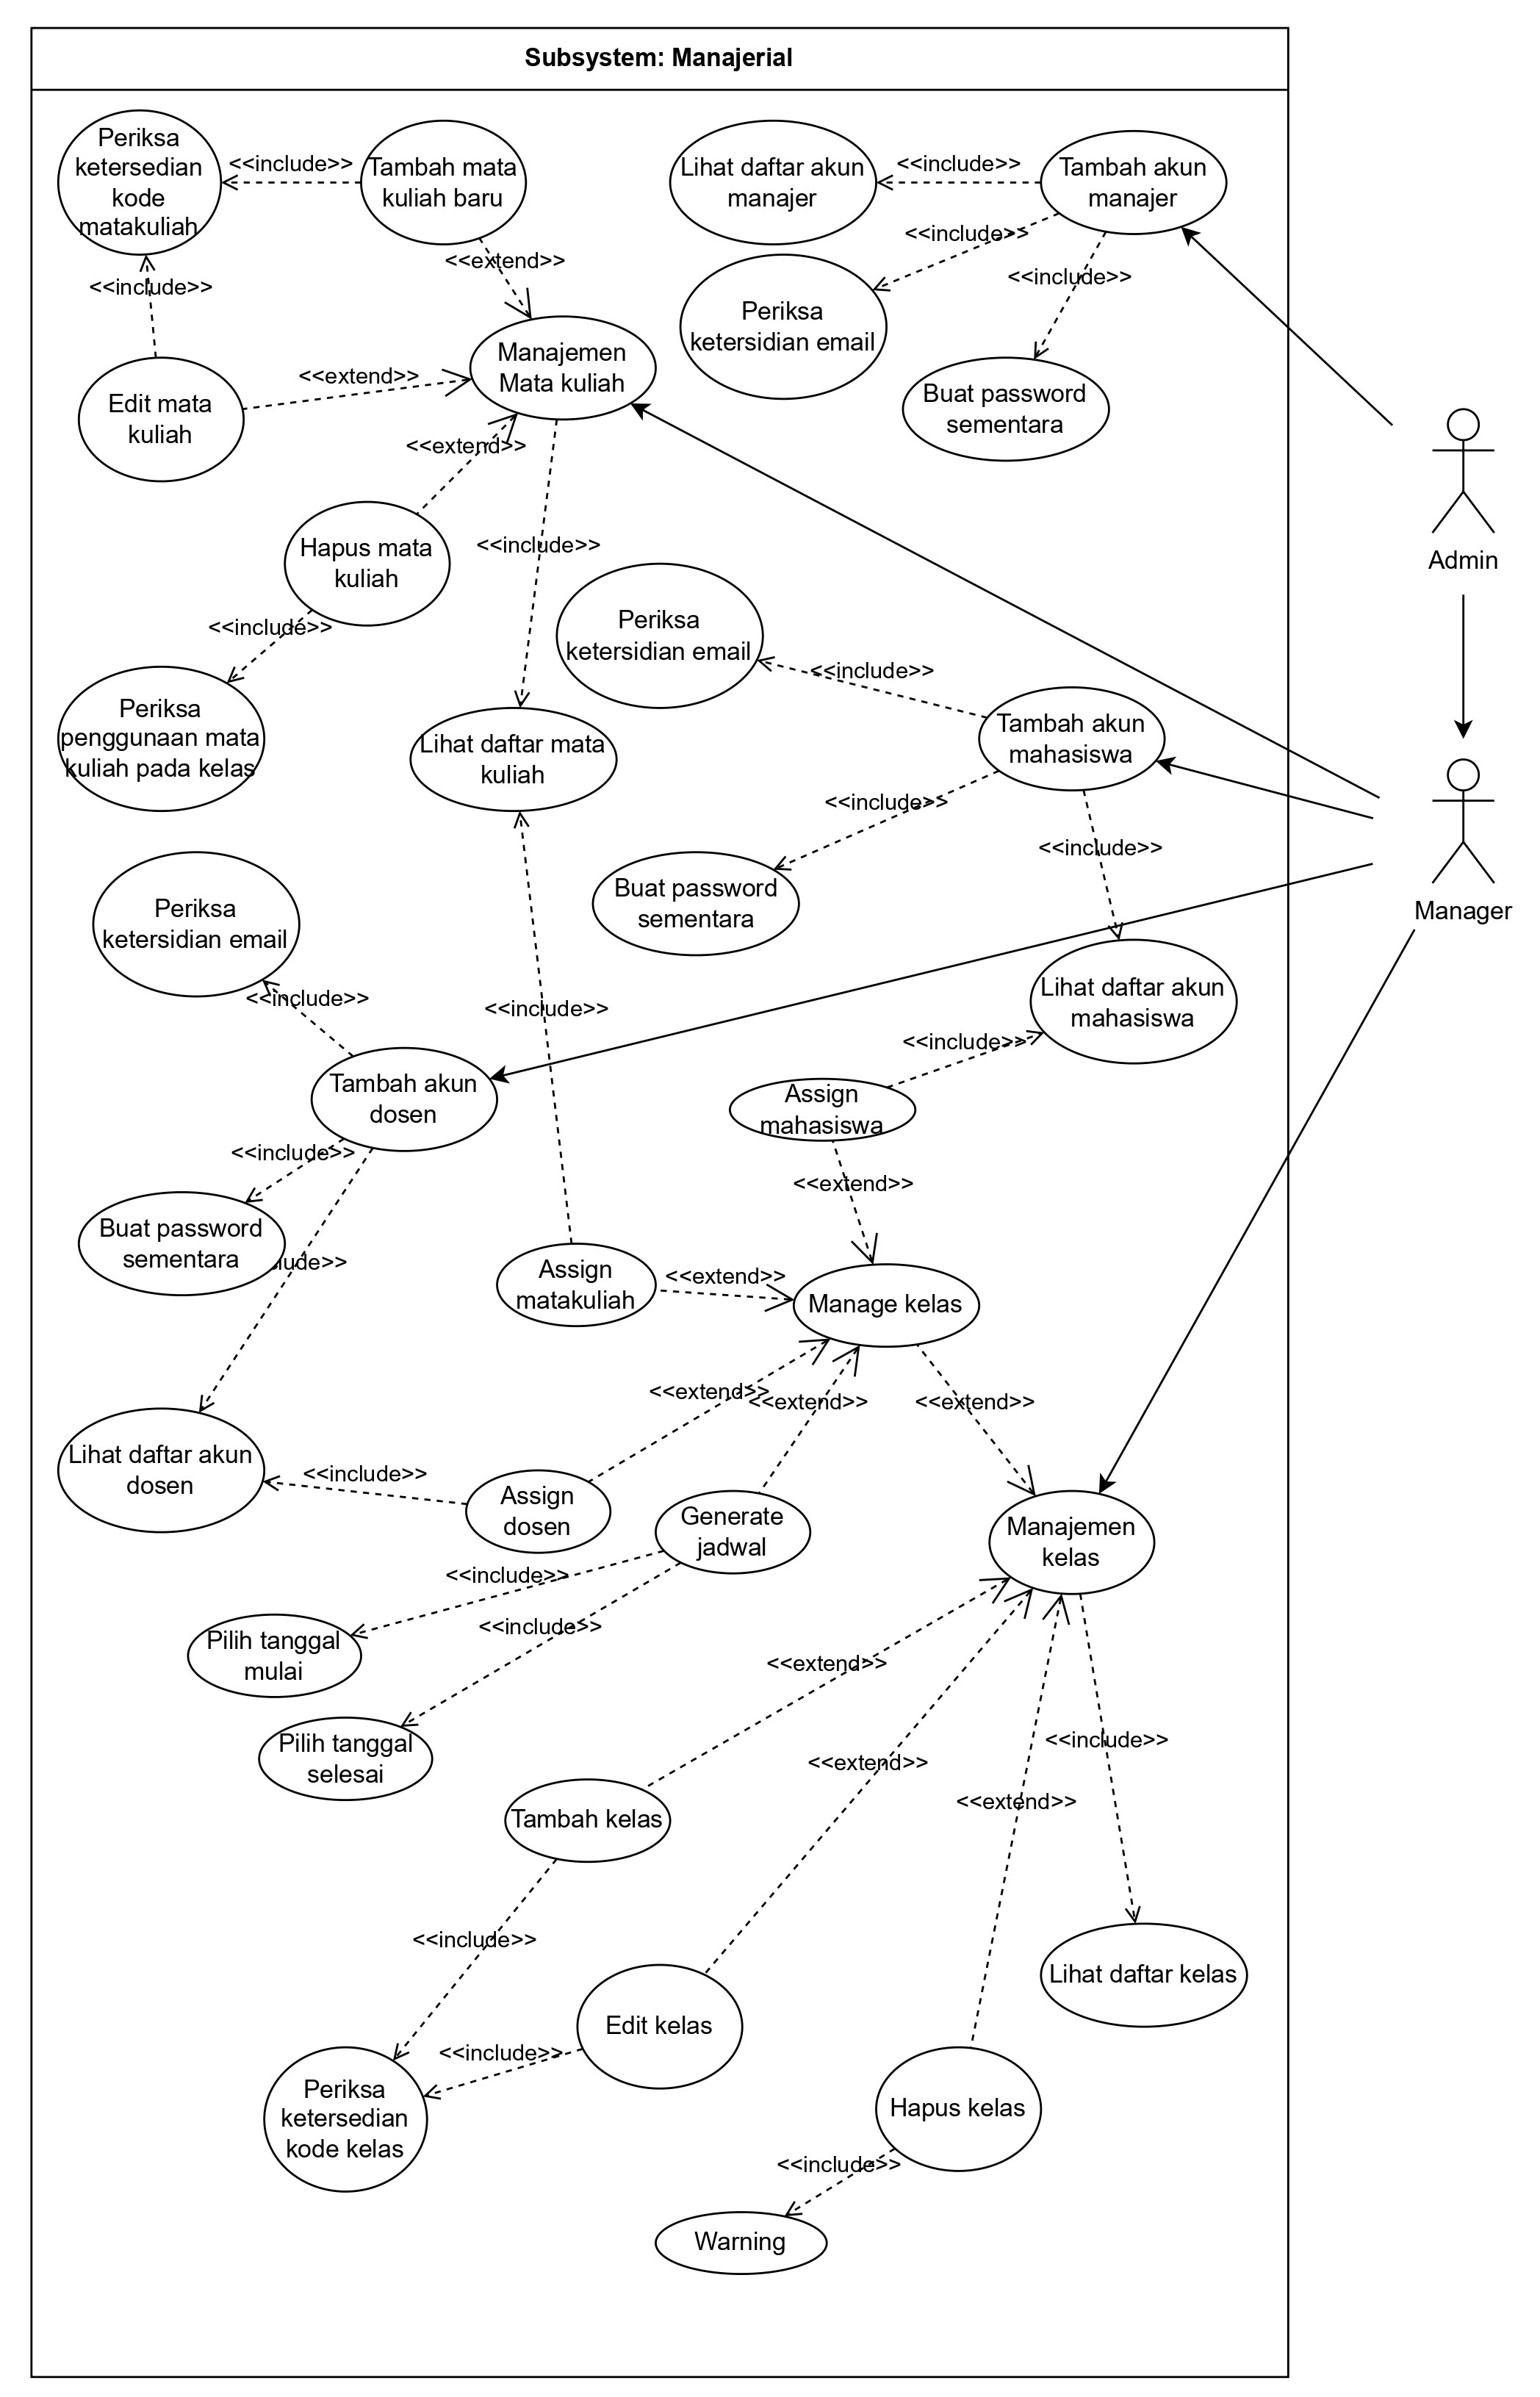
\includegraphics[width=0.8\textwidth]{USECASE/usecasemanajer.jpg}
  \caption{Use Case Manajerial}
  \label{fig:use_case_manajerial}
\end{figure}

\subsubsection{Penjelasan Use Case Manajerial}

Subsystem Manajerial merupakan salah satu bagian inti dalam sistem informasi akademik yang berfungsi untuk mengelola berbagai aspek manajemen perkuliahan, akun pengguna, serta pengaturan kelas dan jadwal. Pada diagram use case \ref{fig:use_case_manajerial} di atas, subsystem ini melibatkan dua aktor utama, yaitu Admin dan Manager, yang memiliki peran berbeda dalam menjalankan fungsionalitas sistem.

\subsubsection{Aktor dan Peran}

\begin{itemize}
  \item \textbf{Admin}: Bertanggung jawab atas pengelolaan akun manajer, dosen, dan mahasiswa, serta memastikan integritas data dan keamanan sistem. Admin dapat menambah akun baru, memeriksa ketersediaan email, dan membuat password sementara untuk pengguna baru.
  \item \textbf{Manager}: Berperan dalam pengelolaan mata kuliah, kelas, dan penjadwalan. Manager dapat menambah, mengedit, dan menghapus mata kuliah serta kelas, mengatur jadwal, dan melakukan assign dosen maupun mahasiswa ke kelas tertentu.
\end{itemize}

\subsubsection{Fitur Utama Subsystem Manajerial}

\begin{enumerate}
  \item \textbf{Manajemen Mata Kuliah:} Fitur ini memungkinkan admin dan manager untuk menambah mata kuliah baru, mengedit, dan menghapus mata kuliah yang sudah ada. Setiap penambahan atau perubahan mata kuliah akan melalui proses validasi, seperti pemeriksaan ketersediaan kode mata kuliah dan penggunaan mata kuliah pada kelas yang sudah berjalan. Hal ini bertujuan untuk menjaga konsistensi data dan mencegah duplikasi atau konflik dalam penjadwalan.
  \item \textbf{Manajemen Akun Pengguna:} Admin dapat menambah akun manajer, dosen, dan mahasiswa. Proses penambahan akun melibatkan pemeriksaan ketersediaan email untuk memastikan tidak ada duplikasi, serta pembuatan password sementara yang dapat diganti oleh pengguna setelah login pertama. Admin juga dapat melihat daftar akun yang sudah terdaftar untuk memudahkan monitoring dan pengelolaan.
  \item \textbf{Manajemen Kelas:} Manager memiliki akses untuk menambah, mengedit, dan menghapus kelas. Setiap kelas yang dibuat harus memiliki kode unik yang diverifikasi oleh sistem. Selain itu, manager dapat melakukan assign dosen dan mahasiswa ke kelas tertentu, serta mengatur jadwal perkuliahan dengan memilih tanggal mulai dan selesai. Fitur generate jadwal membantu manager dalam menyusun jadwal yang optimal dan menghindari bentrok antar kelas.
  \item \textbf{Assign Dosen dan Mahasiswa:} Fitur ini memungkinkan manager untuk mengatur siapa saja dosen dan mahasiswa yang akan mengikuti kelas tertentu. Proses assign dilakukan dengan memperhatikan ketersediaan dosen dan mahasiswa, serta memastikan bahwa tidak ada jadwal yang bertabrakan. Dengan adanya fitur ini, proses pengelolaan kelas menjadi lebih terstruktur dan efisien.
  \item \textbf{Validasi dan Warning:} Setiap proses penambahan atau perubahan data, seperti mata kuliah, kelas, dan akun, akan melalui tahap validasi. Jika ditemukan masalah, seperti kode yang sudah digunakan atau email yang sudah terdaftar, sistem akan memberikan warning kepada pengguna. Hal ini penting untuk menjaga integritas data dan mencegah kesalahan yang dapat berdampak pada proses akademik.
\end{enumerate}


\subsubsection{Alur Interaksi Use Case}

Pada diagram use case \ref{fig:use_case_manajerial} diatas, terlihat adanya relasi <<include>> dan <<extend>> antar fitur. Relasi <<include>> menunjukkan bahwa suatu proses selalu melibatkan proses lain, misalnya setiap penambahan akun pasti melibatkan pemeriksaan ketersediaan email dan pembuatan password sementara. Relasi <<extend>> menunjukkan bahwa suatu proses dapat diperluas dengan fitur tambahan, seperti manajemen kelas yang dapat diperluas dengan fitur generate jadwal atau warning jika terjadi masalah.

\subsubsection{Keamanan dan Efisiensi}

Subsystem Manajerial dirancang dengan memperhatikan aspek keamanan, seperti validasi data dan pembuatan password sementara, serta efisiensi dalam pengelolaan kelas dan jadwal. Dengan adanya fitur-fitur ini, proses administrasi akademik dapat berjalan lebih lancar, terstruktur, dan minim kesalahan.

\subsubsection{Contoh Skenario Penggunaan}

\begin{enumerate}
  \item \textbf{Penambahan Mata Kuliah Baru}: Manager mengakses fitur tambah mata kuliah, memasukkan data mata kuliah, sistem memeriksa ketersediaan kode, jika tersedia maka mata kuliah ditambahkan ke database.
  \item \textbf{Assign Dosen ke Kelas}: Manager memilih kelas yang akan di-assign, memilih dosen yang tersedia, sistem memeriksa jadwal dosen, jika tidak bentrok maka dosen di-assign ke kelas tersebut.
  \item \textbf{Penambahan Akun Mahasiswa}: Admin mengakses fitur tambah akun mahasiswa, memasukkan data mahasiswa, sistem memeriksa email, jika belum terdaftar maka akun dibuat dan password sementara diberikan.
  \item \textbf{Generate Jadwal Kelas}: Manager mengatur jadwal kelas dengan memilih tanggal mulai dan selesai, sistem memeriksa ketersediaan waktu, jika tidak bentrok maka jadwal dibuat dan ditampilkan pada daftar kelas.
\end{enumerate}

\subsubsection{Kesimpulan}

Subsystem Manajerial merupakan komponen penting dalam sistem informasi akademik yang mendukung proses administrasi dan pengelolaan data secara terintegrasi. Dengan fitur-fitur yang lengkap dan terstruktur, subsystem ini membantu admin dan manager dalam menjalankan tugasnya secara efisien, aman, dan akurat. Validasi data, warning, serta relasi antar fitur memastikan bahwa setiap proses berjalan sesuai prosedur dan meminimalisir terjadinya kesalahan. Dengan demikian, subsystem manajerial berperan besar dalam mendukung kelancaran operasional akademik di institusi pendidikan.


% Subsystem login dan usermanajement
\subsection{Subsystem: Login dan User Management}
\begin{figure}[H]
  \centering
  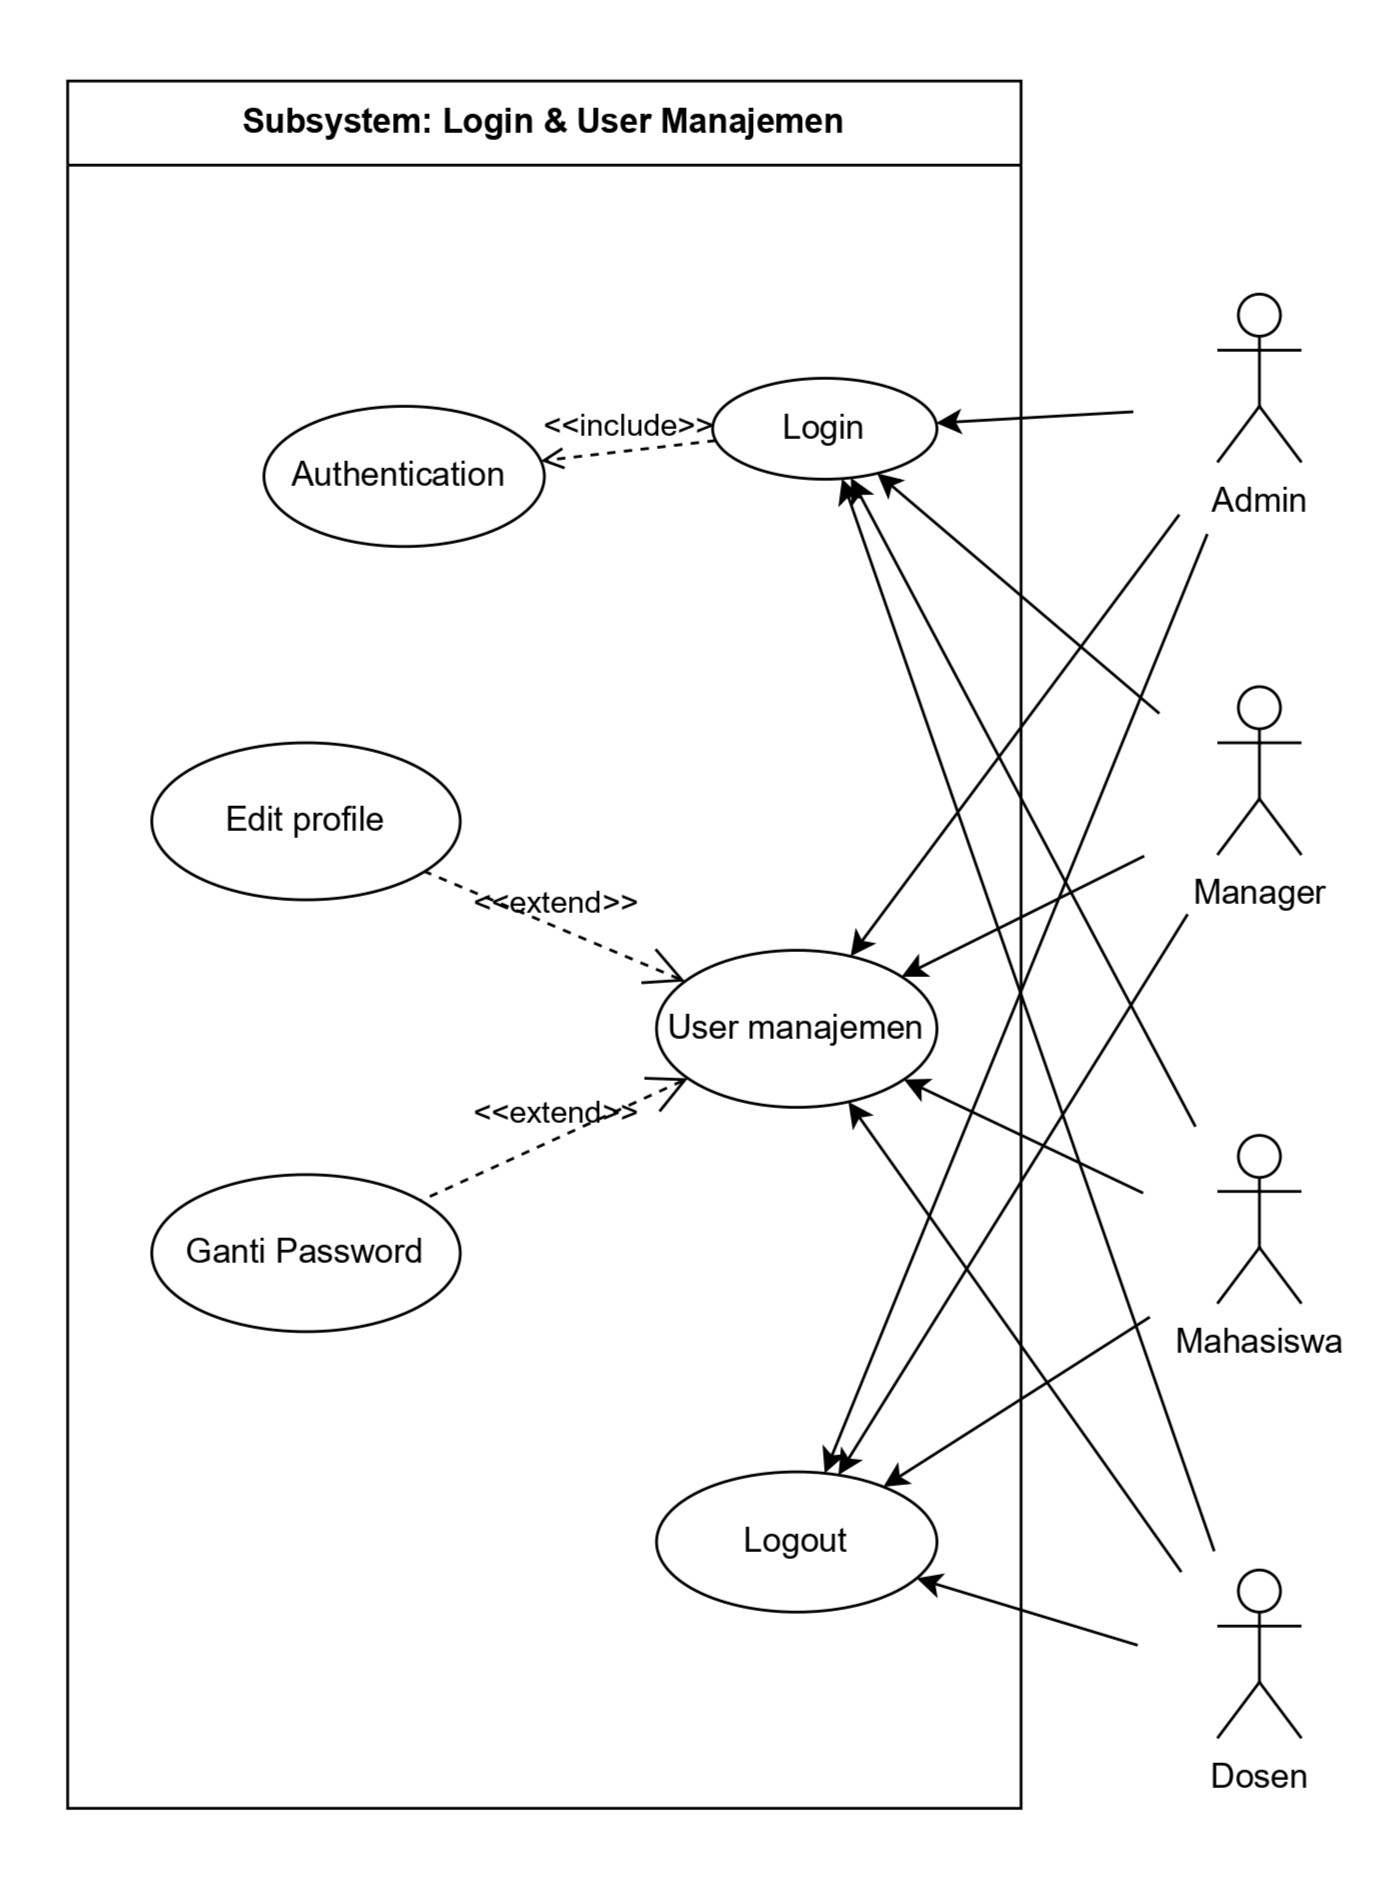
\includegraphics[width=0.8\textwidth]{USECASE/usecaselogin.jpg}
  \caption{Use Case Login dan User Management}
  \label{fig:use_case_login}
\end{figure}

\subsubsection{Penjelasan Use Case Login dan User Management}

Subsystem Login dan User Management merupakan bagian fundamental dari sistem informasi akademik yang bertanggung jawab atas proses autentikasi, pengelolaan identitas pengguna, serta keamanan akses ke seluruh fitur sistem. Pada diagram use case \ref{fig:use_case_login}, subsystem ini melibatkan empat aktor utama, yaitu Admin, Manager, Mahasiswa, dan Dosen, yang semuanya berinteraksi dengan sistem untuk mengakses, mengelola, dan memperbarui data akun mereka.

\subsubsection{Aktor dan Peran}

\begin{itemize}
  \item \textbf{Admin}: Memiliki hak akses penuh untuk mengelola akun seluruh pengguna, melakukan reset password, dan memastikan keamanan sistem.
  \item \textbf{Manager}: Mengelola akun dosen dan mahasiswa, serta dapat memperbarui profil dan password sendiri.
  \item \textbf{Mahasiswa}: Mengakses sistem untuk melihat data akademik, memperbarui profil, dan mengganti password.
  \item \textbf{Dosen}: Mengelola data pribadi, mengakses jadwal, dan melakukan perubahan password sesuai kebutuhan.
\end{itemize}

\subsubsection{Fitur Utama Subsystem Login dan User Management}

\begin{enumerate}
  \item \textbf{Login dan Authentication:} Fitur ini merupakan pintu masuk utama ke sistem. Setiap pengguna harus melakukan login dengan kredensial yang valid. Proses login selalu melibatkan autentikasi, yaitu verifikasi username dan password, serta validasi status akun. Jika autentikasi berhasil, pengguna dapat mengakses fitur sesuai hak aksesnya.
  \item \textbf{User Management:} Setelah login, pengguna dapat mengelola data profil, seperti nama, email, dan informasi kontak. Admin dapat mengelola seluruh akun, termasuk menambah, mengedit, dan menghapus akun pengguna lain. Fitur ini juga mendukung pengelolaan hak akses dan peran pengguna.
  \item \textbf{Edit Profile:} Pengguna dapat memperbarui data pribadi mereka, seperti nama, email, dan foto profil. Fitur ini penting untuk menjaga data tetap akurat dan up-to-date. Proses edit profile dilakukan melalui relasi <<extend>> pada user management.
  \item \textbf{Ganti Password:} Untuk menjaga keamanan, pengguna dapat mengganti password secara mandiri. Proses ini juga dilakukan melalui relasi <<extend>> pada user management. Admin dapat melakukan reset password jika pengguna lupa atau terjadi masalah keamanan.
  \item \textbf{Logout:} Fitur logout memastikan bahwa sesi pengguna berakhir dengan aman, sehingga mencegah akses tidak sah ke data pribadi dan fitur sistem. Semua aktor dapat melakukan logout setelah selesai menggunakan sistem.
\end{enumerate}

\subsubsection{Alur Interaksi Use Case}

Pada diagram use case, terlihat bahwa proses login selalu melibatkan autentikasi (<<include>>), sedangkan user management dapat diperluas dengan fitur edit profile dan ganti password (<<extend>>). Setiap aktor dapat melakukan login, mengelola akun, dan logout sesuai dengan hak akses yang dimiliki. Admin memiliki hak istimewa untuk mengelola seluruh akun dan melakukan reset password, sedangkan pengguna lain hanya dapat mengelola akun mereka sendiri.

\subsubsection{Keamanan dan Efisiensi}

Subsystem ini dirancang dengan fokus pada keamanan data dan efisiensi akses. Proses autentikasi menggunakan enkripsi password dan validasi multi-level untuk mencegah akses tidak sah. Fitur ganti password dan edit profile memberikan fleksibilitas bagi pengguna untuk menjaga keamanan dan akurasi data. Logout yang aman memastikan tidak ada sesi yang terbuka setelah pengguna selesai menggunakan sistem.

\subsubsection{Contoh Skenario Penggunaan}

\begin{enumerate}
  \item \textbf{Login Mahasiswa}: Mahasiswa memasukkan username dan password, sistem melakukan autentikasi, jika berhasil mahasiswa dapat mengakses data akademik dan fitur lain sesuai hak akses.
  \item \textbf{Edit Profile Dosen}: Dosen login ke sistem, mengakses fitur edit profile, memperbarui data pribadi, dan menyimpan perubahan. Sistem memvalidasi data dan memperbarui database.
  \item \textbf{Ganti Password Manager}: Manager login, memilih fitur ganti password, memasukkan password lama dan baru, sistem memvalidasi dan mengupdate password di database.
  \item \textbf{Logout Admin}: Setelah selesai mengelola akun, admin melakukan logout untuk mengakhiri sesi dan menjaga keamanan sistem.
\end{enumerate}

\subsubsection{Kesimpulan}

Subsystem Login dan User Management adalah salah satu fondasi utama dalam sistem informasi akademik yang memastikan setiap pengguna dapat mengakses fitur sesuai haknya dengan aman dan efisien. Dengan fitur login, autentikasi, pengelolaan akun, edit profile, ganti password, dan logout, subsystem ini mendukung kelancaran operasional serta menjaga integritas dan keamanan data seluruh pengguna. Relasi antar fitur dan aktor pada diagram use case memastikan bahwa setiap proses berjalan sesuai prosedur dan meminimalisir risiko keamanan. Dengan demikian, subsystem ini sangat penting untuk mendukung aktivitas akademik dan administrasi di institusi pendidikan modern.

%  Subsystem sistem infomasi
\subsection{Subsystem: Sistem Informasi}
\begin{figure}[H]
  \centering
  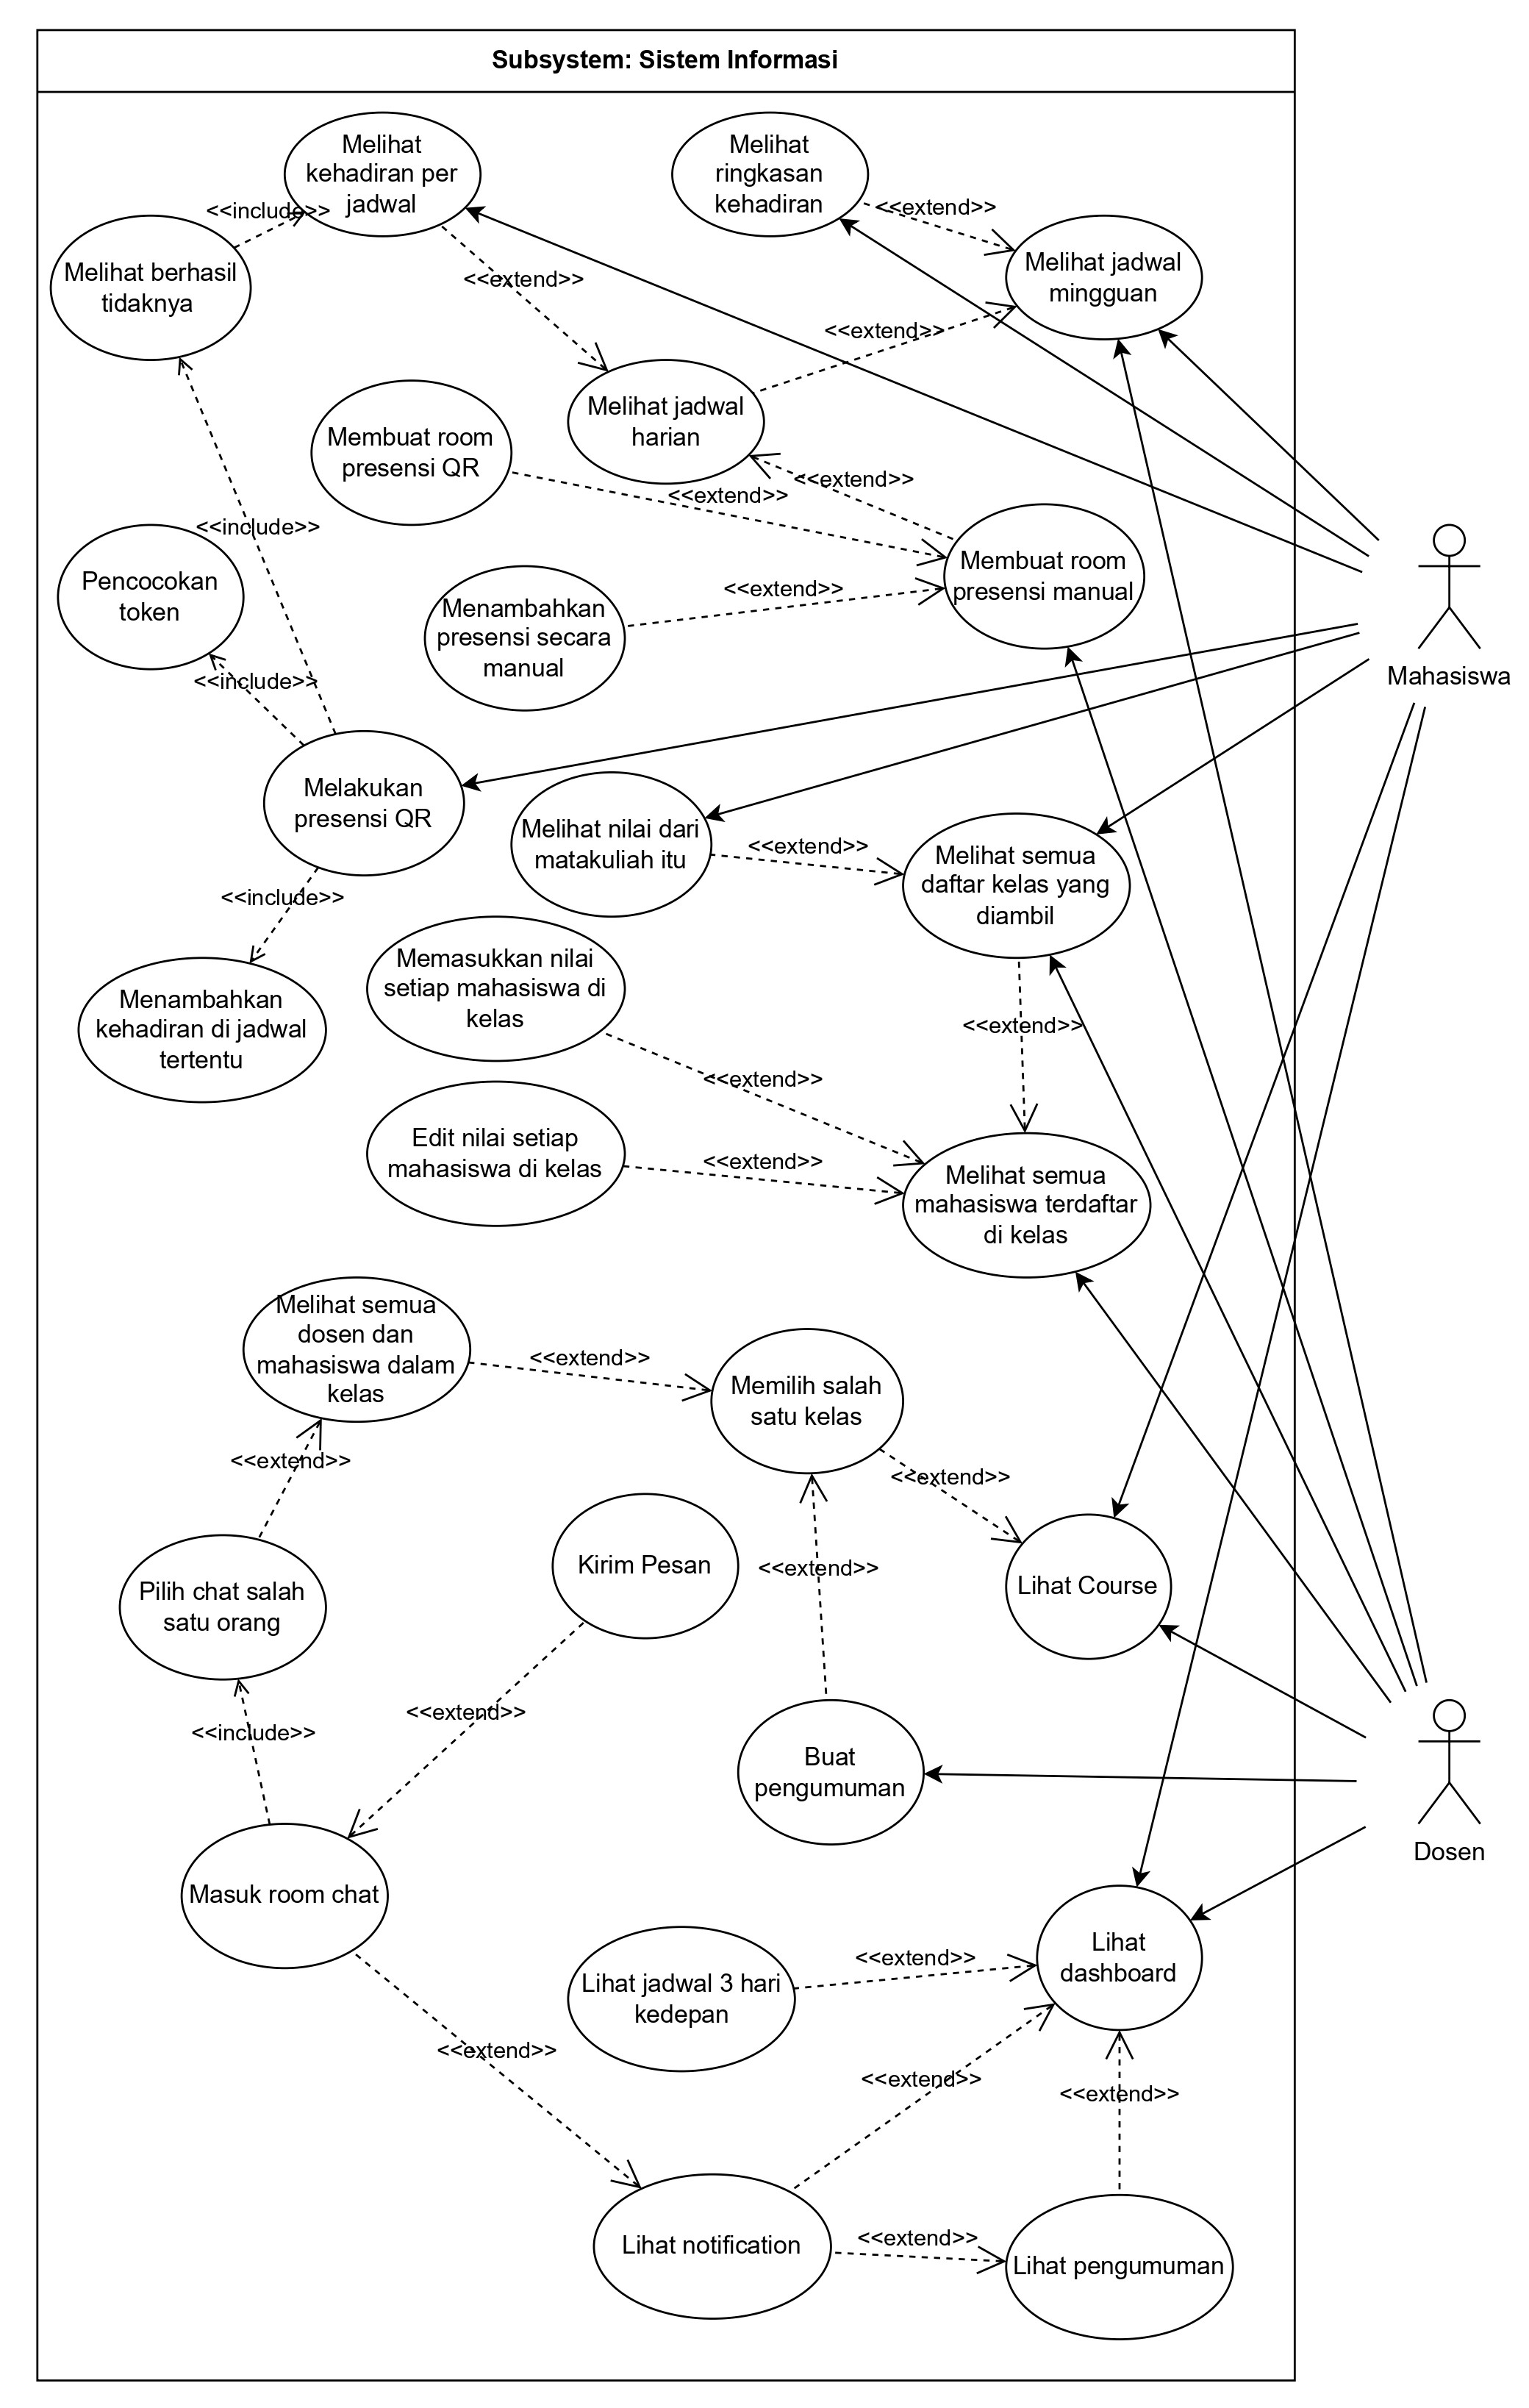
\includegraphics[width=0.8\textwidth]{USECASE/usecaseSistemInformasi.jpg}
  \caption{Use Case Sistem Informasi}
  \label{fig:use_case_sistem_informasi}
\end{figure}

\subsubsection{Penjelasan Use Case Sistem Informasi}

Subsystem Sistem Informasi adalah bagian yang sangat penting dalam sistem akademik modern, karena menyediakan berbagai fitur yang mendukung proses pembelajaran, komunikasi, dan monitoring aktivitas akademik secara digital. Pada diagram use case \ref{fig:use_case_sistem_informasi}, subsystem ini melibatkan dua aktor utama, yaitu Mahasiswa dan Dosen, yang berinteraksi dengan sistem untuk mengakses informasi, melakukan presensi, melihat nilai, berkomunikasi, dan mendapatkan notifikasi terkait aktivitas akademik.

\subsubsection{Aktor dan Peran}

\begin{itemize}
  \item \textbf{Mahasiswa}: Mengakses sistem untuk melihat jadwal, melakukan presensi, melihat nilai, berkomunikasi dengan dosen dan sesama mahasiswa, serta menerima pengumuman dan notifikasi.
  \item \textbf{Dosen}: Mengelola presensi, memasukkan dan mengedit nilai mahasiswa, membuat pengumuman, serta berkomunikasi dengan mahasiswa melalui chat dan notifikasi.
\end{itemize}

\subsubsection{Fitur Utama Subsystem Sistem Informasi}

\begin{enumerate}
  \item \textbf{Presensi QR dan Manual:} Fitur ini memungkinkan mahasiswa untuk melakukan presensi secara digital menggunakan QR code atau secara manual. Dosen dapat membuat room presensi QR atau manual, dan mahasiswa melakukan presensi dengan mencocokkan token atau memasukkan data secara manual. Sistem akan memvalidasi kehadiran dan mencatat status presensi setiap mahasiswa.
  \item \textbf{Monitoring Kehadiran:} Mahasiswa dapat melihat kehadiran per jadwal, ringkasan kehadiran, dan status presensi mingguan maupun harian. Dosen dapat menambahkan kehadiran di jadwal tertentu dan memantau kehadiran mahasiswa secara real-time.
  \item \textbf{Manajemen Nilai:} Dosen dapat memasukkan dan mengedit nilai setiap mahasiswa di kelas. Mahasiswa dapat melihat nilai dari setiap mata kuliah yang diambil. Proses ini terintegrasi dengan daftar kelas dan daftar mahasiswa yang terdaftar di kelas tersebut.
  \item \textbf{Manajemen Kelas dan Course:} Mahasiswa dapat melihat semua daftar kelas yang diambil dan semua mahasiswa yang terdaftar di kelas. Dosen dapat melihat semua dosen dan mahasiswa dalam kelas, serta mengelola course yang diampu.
  \item \textbf{Jadwal dan Dashboard:} Mahasiswa dan dosen dapat melihat jadwal harian, mingguan, dan 3 hari ke depan. Dashboard menyediakan ringkasan aktivitas, jadwal, pengumuman, dan notifikasi yang relevan dengan peran masing-masing aktor.
  \item \textbf{Komunikasi dan Pengumuman:} Fitur chat memungkinkan mahasiswa dan dosen untuk berkomunikasi secara langsung, baik dalam room chat maupun secara personal. Dosen dapat membuat pengumuman yang akan muncul di dashboard dan notifikasi mahasiswa.
  \item \textbf{Notifikasi:} Sistem mengirimkan notifikasi terkait jadwal, pengumuman, dan aktivitas penting lainnya agar mahasiswa dan dosen selalu mendapatkan update terbaru.
\end{enumerate}

\subsubsection{Alur Interaksi Use Case}

Pada diagram use case, terdapat relasi <<include>> dan <<extend>> yang menggambarkan keterkaitan antar fitur. Misalnya, proses melakukan presensi QR selalu melibatkan pencocokan token dan validasi kehadiran. Fitur melihat jadwal harian dan mingguan merupakan perluasan dari fitur monitoring kehadiran. Proses memasukkan dan mengedit nilai mahasiswa di kelas akan terhubung dengan fitur melihat daftar kelas dan mahasiswa yang terdaftar.

Komunikasi antar mahasiswa dan dosen difasilitasi melalui fitur chat, room chat, dan pengumuman. Setiap pengumuman yang dibuat dosen akan muncul di dashboard dan notifikasi mahasiswa, sehingga informasi penting tidak terlewatkan.

\subsubsection{Keamanan dan Efisiensi}

Subsystem ini dirancang untuk memastikan keamanan data akademik, kehadiran, dan nilai mahasiswa. Proses presensi menggunakan QR code dan token untuk mencegah kecurangan. Data nilai dan kehadiran disimpan secara terpusat dan hanya dapat diakses oleh aktor yang berwenang. Notifikasi dan dashboard membantu meningkatkan efisiensi komunikasi dan monitoring aktivitas akademik.

\subsubsection{Contoh Skenario Penggunaan}

\begin{enumerate}
  \item \textbf{Presensi QR Mahasiswa}: Mahasiswa masuk ke room presensi QR, melakukan scan QR code, sistem mencocokkan token dan mencatat kehadiran. Mahasiswa dapat melihat status kehadiran pada jadwal tersebut.
  \item \textbf{Dosen Memasukkan Nilai}: Dosen memilih kelas, memasukkan nilai setiap mahasiswa, dan menyimpan data. Mahasiswa dapat melihat nilai yang telah diinput pada dashboard mereka.
  \item \textbf{Mahasiswa Melihat Jadwal}: Mahasiswa mengakses dashboard untuk melihat jadwal harian, mingguan, dan 3 hari ke depan, serta mendapatkan notifikasi jika ada perubahan jadwal atau pengumuman baru.
  \item \textbf{Chat dan Pengumuman}: Mahasiswa dan dosen masuk ke room chat, memilih salah satu kelas, dan mengirim pesan atau membuat pengumuman yang akan diterima oleh seluruh anggota kelas.
\end{enumerate}

\subsubsection{Kesimpulan}

Subsystem Sistem Informasi merupakan tulang punggung digitalisasi proses akademik di institusi pendidikan. Dengan fitur presensi digital, monitoring kehadiran, manajemen nilai, jadwal, dashboard, komunikasi, dan notifikasi, subsystem ini mendukung kelancaran pembelajaran dan administrasi akademik secara efisien dan aman. Relasi antar fitur dan aktor pada diagram use case memastikan setiap proses berjalan terintegrasi dan sesuai prosedur, sehingga mahasiswa dan dosen dapat fokus pada aktivitas akademik tanpa hambatan teknis. Dengan demikian, subsystem sistem informasi sangat penting untuk mendukung transformasi digital di lingkungan pendidikan modern.

\section{Activity Diagram}


\subsection{Activity Diagram Chat}
\begin{figure}[H]
  \centering
  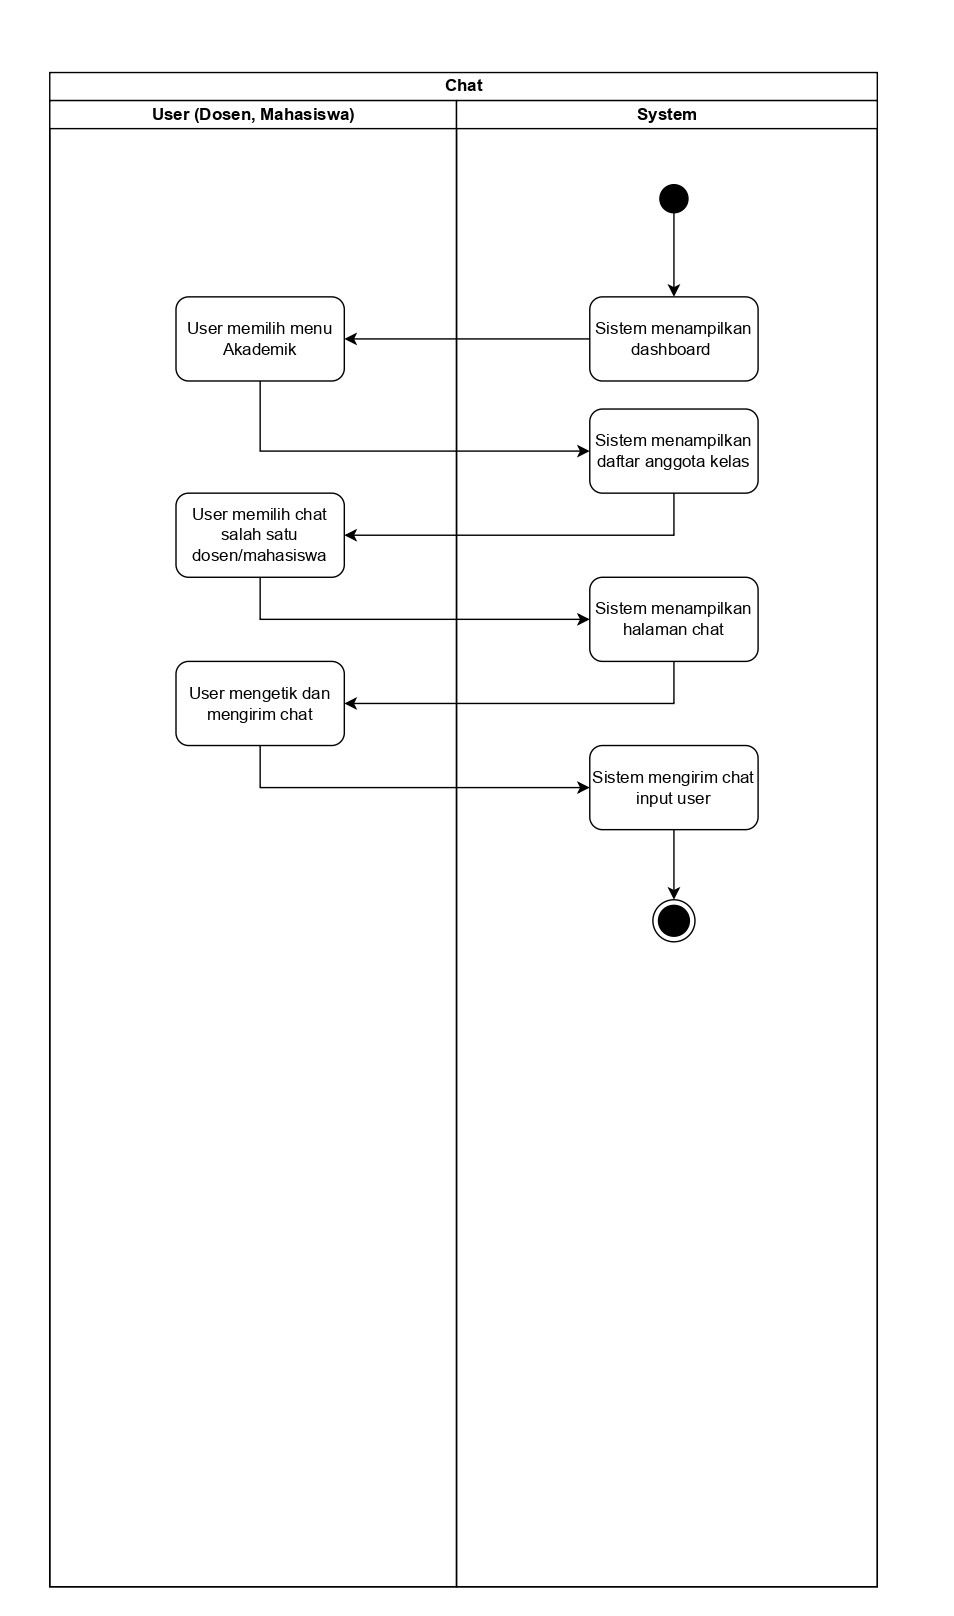
\includegraphics[width=0.8\textwidth]{Activity Diagram/Chat.jpg}
  \caption{Activity Diagram Chat}
  \label{fig:activity_chat}
\end{figure}

\subsubsection{Penjelasan Activity Diagram Chat}
Activity Diagram Chat pada sistem informasi akademik \ref{fig:activity_chat} ini menggambarkan alur komunikasi digital antara pengguna, yaitu dosen dan mahasiswa, dengan sistem. Diagram ini terdiri dari dua swimlane utama, yaitu swimlane untuk User (Dosen, Mahasiswa) dan swimlane untuk System, yang memperjelas peran masing-masing dalam proses komunikasi.

Proses dimulai ketika user memilih menu Akademik pada dashboard aplikasi. Sistem merespons dengan menampilkan dashboard utama yang berisi berbagai fitur akademik, termasuk daftar anggota kelas. Tahap ini penting karena memungkinkan user untuk mengakses informasi terkini mengenai kelas dan anggota yang terlibat, sehingga komunikasi dapat dilakukan secara lebih terarah.

Selanjutnya, user dapat memilih salah satu anggota kelas, baik dosen maupun mahasiswa, untuk memulai percakapan chat. Sistem kemudian menampilkan halaman chat yang relevan, di mana user dapat melihat riwayat percakapan sebelumnya dan mulai berinteraksi. Pada tahap ini, sistem memastikan bahwa hanya user yang berwenang dan terdaftar dalam kelas tersebut yang dapat mengakses fitur chat, sehingga privasi dan keamanan komunikasi tetap terjaga.

Setelah halaman chat terbuka, user dapat mengetik pesan dan mengirimkannya melalui aplikasi. Sistem akan menerima input chat dari user, memprosesnya, dan mengirimkan pesan tersebut ke penerima yang dituju. Proses pengiriman chat ini dilakukan secara real-time, sehingga komunikasi antara dosen dan mahasiswa dapat berlangsung dengan cepat dan efisien. Sistem juga dapat memberikan notifikasi kepada penerima jika ada pesan baru yang masuk, baik melalui aplikasi maupun email, tergantung pada pengaturan notifikasi yang dipilih oleh user.

Diagram \ref{fig:activity_chat} ini juga memperlihatkan adanya validasi dan pengelolaan hak akses pada setiap tahap. Misalnya, sebelum user dapat mengirim chat, sistem akan memeriksa apakah user tersebut memang memiliki hak untuk berkomunikasi dengan anggota kelas yang dipilih. Jika validasi berhasil, proses pengiriman chat dilanjutkan; jika tidak, sistem akan menampilkan pesan error atau peringatan kepada user.

Secara keseluruhan, Activity Diagram Chat \ref{fig:activity_chat} ini menunjukkan bagaimana sistem mendukung komunikasi akademik yang terstruktur dan aman. Dengan adanya fitur chat, dosen dan mahasiswa dapat bertukar informasi, berdiskusi mengenai materi perkuliahan, menyampaikan pertanyaan, atau memberikan umpan balik secara langsung. Proses yang digambarkan dalam diagram ini juga memastikan bahwa setiap interaksi tercatat dengan baik, sehingga dapat digunakan sebagai referensi atau bukti komunikasi di kemudian hari.

Fitur chat yang terintegrasi dalam sistem informasi akademik sangat penting untuk mendukung pembelajaran digital, mempercepat penyebaran informasi, dan meningkatkan kolaborasi antara dosen dan mahasiswa. Dengan alur yang jelas dan validasi yang ketat, sistem dapat meminimalisir risiko kesalahan komunikasi, menjaga privasi, serta meningkatkan efisiensi proses akademik secara keseluruhan.

\subsubsection{Penjelasan Activity Diagram Chat}

\subsection{Activity Diagram Dosen}
\begin{figure}[H]
  \centering
  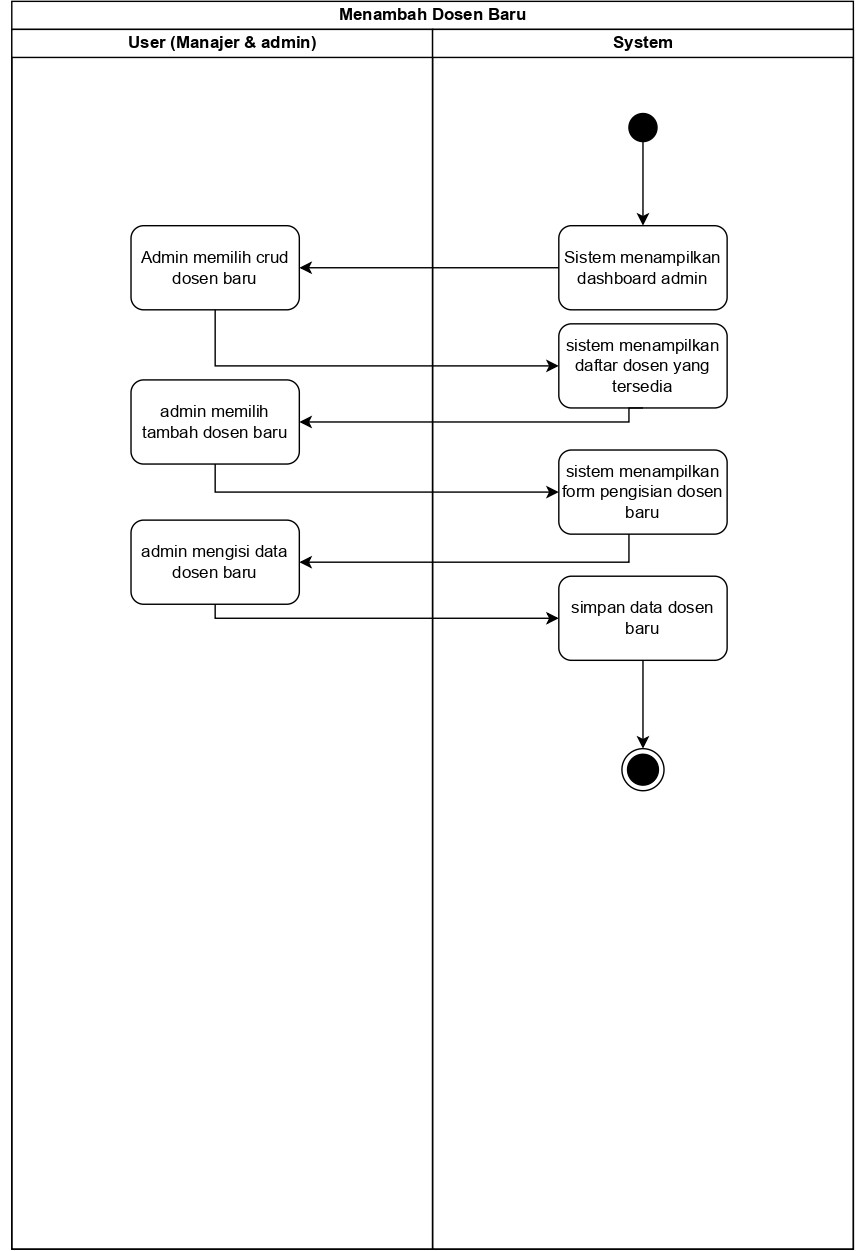
\includegraphics[width=0.8\textwidth]{Activity Diagram/Dosen.jpg}
  \caption{Activity Diagram Dosen}
  \label{fig:activity_dosen}
\end{figure}

\subsubsection{Penjelasan Activity Diagram Dosen}
Activity Diagram Dosen pada sistem informasi akademik ini \ref{fig:activity_dosen} secara khusus menggambarkan proses penambahan dosen baru oleh user yang berperan sebagai manajer atau admin. Diagram ini terdiri dari dua swimlane utama, yaitu swimlane untuk User (Manajer dan Admin) dan swimlane untuk System, yang memperjelas interaksi dan tanggung jawab masing-masing pihak dalam proses administrasi dosen.

Proses dimulai ketika admin mengakses dashboard admin dan memilih menu CRUD dosen baru. Sistem merespons dengan menampilkan dashboard yang berisi daftar dosen yang sudah tersedia di database. Tahap ini penting untuk memberikan gambaran kepada admin mengenai data dosen yang sudah ada, sehingga dapat menghindari duplikasi dan memudahkan monitoring data dosen.

Selanjutnya, admin memilih opsi tambah dosen baru. Sistem kemudian menampilkan form pengisian data dosen baru yang harus diisi oleh admin. Form ini biasanya berisi data identitas dosen seperti nama, NIP, email, program studi, dan informasi lain yang relevan. Pada tahap ini, sistem melakukan validasi awal terhadap data yang diinput, seperti pengecekan format email, ketersediaan NIP, dan kelengkapan data agar tidak terjadi kesalahan atau kekurangan informasi.

Setelah admin mengisi data dosen baru secara lengkap dan benar, sistem akan menyimpan data tersebut ke dalam database. Proses penyimpanan ini dilakukan secara otomatis setelah admin menekan tombol simpan pada form. Sistem juga dapat memberikan notifikasi atau konfirmasi bahwa data dosen baru telah berhasil ditambahkan. Jika terjadi error, seperti data duplikat atau format tidak sesuai, sistem akan menampilkan pesan peringatan agar admin dapat memperbaiki input sebelum data disimpan.

Diagram \ref{fig:activity_dosen} ini juga menampilkan validasi hak akses, di mana hanya user dengan peran admin atau manajer yang dapat melakukan penambahan dosen baru. Validasi ini penting untuk menjaga keamanan dan integritas data, serta memastikan bahwa proses administrasi dilakukan oleh pihak yang berwenang.

Secara keseluruhan, Activity Diagram Dosen \ref{fig:activity_dosen} ini menunjukkan bagaimana sistem mendukung proses penambahan dosen baru secara terstruktur, efisien, dan aman. Dengan adanya fitur ini, institusi pendidikan dapat memperbarui data dosen secara berkala, menambah dosen baru sesuai kebutuhan, dan menjaga kualitas data akademik. Proses yang digambarkan dalam diagram ini juga memastikan bahwa setiap langkah tercatat dengan baik, sehingga dapat digunakan sebagai referensi atau audit administrasi di kemudian hari.

Fitur penambahan dosen baru yang terintegrasi dalam sistem informasi akademik sangat penting untuk mendukung pengelolaan sumber daya manusia di lingkungan kampus. Dengan alur yang jelas, validasi data yang ketat, dan hak akses yang terjaga, sistem dapat meminimalisir risiko kesalahan input, menjaga keamanan data, serta meningkatkan efisiensi proses administrasi dosen secara keseluruhan.


\subsection{Activity Diagram Kelas}
\begin{figure}[H]
  \centering
  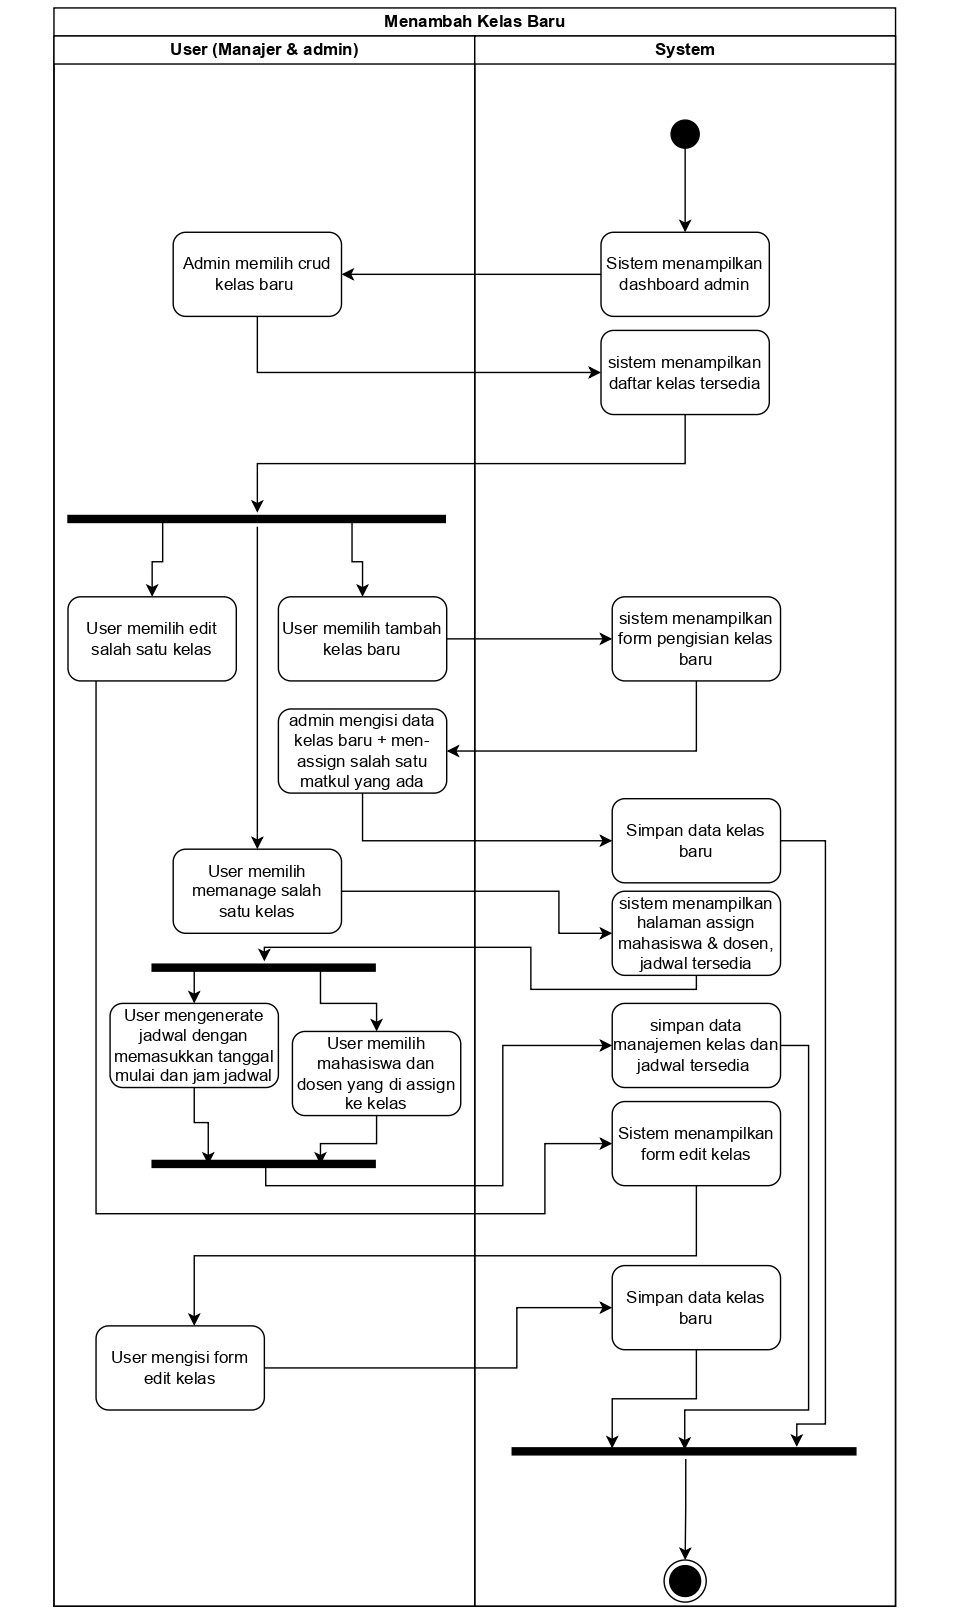
\includegraphics[width=0.8\textwidth]{Activity Diagram/Kelas.jpg}
  \caption{Activity Diagram Kelas}
  \label{fig:activity_kelas}
\end{figure}

\subsubsection{Penjelasan Activity Diagram Kelas}
Activity Diagram Kelas pada sistem informasi akademik ini, seperti yang ditunjukkan pada Gambar~\ref{fig:activity_kelas}, menggambarkan proses lengkap penambahan dan pengelolaan kelas baru oleh user yang berperan sebagai manajer atau admin. Diagram ini terdiri dari dua swimlane utama, yaitu User (Manajer dan Admin) dan System, yang memperjelas interaksi serta tanggung jawab masing-masing pihak dalam proses administrasi kelas.

Proses dimulai ketika admin memilih menu CRUD kelas baru pada dashboard admin. Sistem merespons dengan menampilkan daftar kelas yang sudah tersedia, sehingga admin dapat melihat data kelas yang ada dan menghindari duplikasi. Selanjutnya, admin dapat memilih untuk mengedit kelas yang sudah ada atau menambah kelas baru. Jika memilih tambah kelas baru, sistem akan menampilkan form pengisian data kelas baru yang harus diisi oleh admin, termasuk meng-assign salah satu mata kuliah yang tersedia ke kelas tersebut.

Setelah data kelas baru diisi dan mata kuliah di-assign, sistem akan menyimpan data kelas baru ke database. Proses ini memastikan bahwa setiap kelas yang ditambahkan sudah terintegrasi dengan mata kuliah yang relevan. Selanjutnya, admin dapat memilih untuk memanage salah satu kelas, di mana sistem akan menampilkan halaman assign mahasiswa dan dosen ke kelas serta jadwal yang tersedia. Pada tahap ini, admin dapat memilih mahasiswa dan dosen yang akan mengikuti kelas, serta mengatur jadwal perkuliahan dengan memasukkan tanggal mulai dan jam jadwal.

Sistem kemudian menyimpan data manajemen kelas dan jadwal yang telah diatur, memastikan bahwa semua informasi terkait kelas, peserta, dan jadwal tercatat dengan baik. Jika admin memilih untuk mengedit kelas, sistem akan menampilkan form edit kelas yang dapat diisi untuk memperbarui data kelas sesuai kebutuhan. Setelah form edit kelas diisi, sistem akan menyimpan data kelas yang telah diperbarui ke database.

Diagram~\ref{fig:activity_kelas} juga menampilkan validasi hak akses dan data pada setiap tahap, seperti pengecekan kelengkapan data kelas, validasi jadwal agar tidak bentrok, serta pengecekan status mahasiswa dan dosen yang di-assign ke kelas. Validasi ini penting untuk menjaga integritas data dan memastikan proses administrasi berjalan sesuai prosedur.

Secara keseluruhan, Activity Diagram Kelas pada Gambar~\ref{fig:activity_kelas} menunjukkan bagaimana sistem mendukung proses penambahan, pengelolaan, dan pengeditan kelas secara terstruktur, efisien, dan aman. Dengan adanya fitur ini, institusi pendidikan dapat memperbarui data kelas secara berkala, menambah kelas baru sesuai kebutuhan, dan menjaga kualitas data akademik. Proses yang digambarkan dalam diagram ini juga memastikan bahwa setiap langkah tercatat dengan baik, sehingga dapat digunakan sebagai referensi atau audit administrasi di kemudian hari.

Fitur manajemen kelas yang terintegrasi dalam sistem informasi akademik sangat penting untuk mendukung pengelolaan proses belajar mengajar di lingkungan kampus. Dengan alur yang jelas, validasi data yang ketat, dan hak akses yang terjaga, sistem dapat meminimalisir risiko kesalahan input, menjaga keamanan data, serta meningkatkan efisiensi proses administrasi kelas secara keseluruhan.


\subsection{Activity Diagram Login}
\begin{figure}[H]
  \centering
  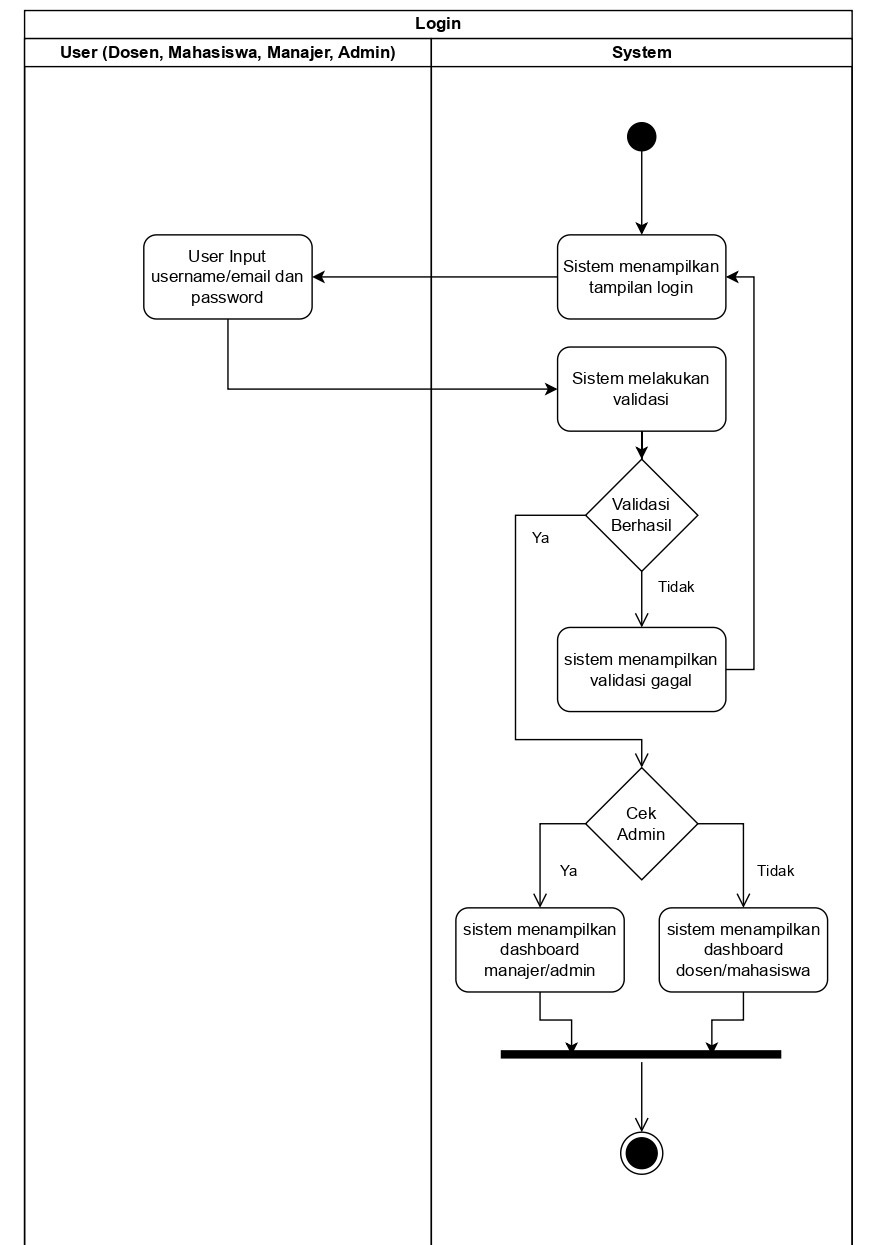
\includegraphics[width=0.8\textwidth]{Activity Diagram/Login.jpg}
  \caption{Activity Diagram Login}
  \label{fig:activity_login}
\end{figure}

\subsubsection{Penjelasan Activity Diagram Login}
Activity Diagram Login pada Gambar~\ref{fig:activity_login} menjabarkan alur proses autentikasi pengguna dalam sistem informasi akademik. Proses dimulai ketika user, baik dosen, mahasiswa, manajer, maupun admin, menginput username/email dan password pada tampilan login yang disediakan oleh sistem. Setelah data diinput, sistem melakukan validasi terhadap kredensial yang dimasukkan. Validasi ini bertujuan untuk memastikan bahwa data yang diberikan sesuai dengan yang terdaftar di database dan belum terjadi kesalahan input.

Jika validasi berhasil, sistem akan melakukan pengecekan role user. Jika user adalah admin atau manajer, sistem akan menampilkan dashboard khusus yang berisi fitur-fitur manajerial dan administrasi. Sebaliknya, jika user adalah dosen atau mahasiswa, sistem akan menampilkan dashboard yang berisi fitur-fitur akademik sesuai peran masing-masing. Jika validasi gagal, sistem akan menampilkan pesan error atau tampilan validasi gagal agar user dapat memperbaiki data yang diinput.

Diagram~\ref{fig:activity_login} juga memperlihatkan pentingnya proses validasi dan pemisahan hak akses yang berdasarkan role. Dengan adanya pemisahan dashboard, sistem dapat memastikan bahwa setiap user hanya dapat mengakses fitur yang relevan dan sesuai dengan otoritasnya. Hal ini sangat penting untuk menjaga keamanan data dan efisiensi operasional sistem.

Beberapa hal penting yang perlu diperhatikan dalam alur login ini adalah penggunaan enkripsi password untuk menjaga keamanan data, serta adanya notifikasi atau feedback yang jelas ketika terjadi kesalahan input. Selain itu, sistem juga harus mampu menangani berbagai skenario login, seperti lupa password, akun tidak aktif, atau user belum terdaftar, dengan memberikan solusi atau petunjuk yang mudah dipahami.

Secara keseluruhan, Activity Diagram Login pada Gambar~\ref{fig:activity_login} memberikan gambaran terstruktur tentang bagaimana proses autentikasi dan otorisasi dilakukan dalam sistem informasi akademik. Dengan alur yang jelas dan validasi yang ketat, sistem dapat meminimalisir risiko akses tidak sah, menjaga privasi data, serta meningkatkan kenyamanan dan efisiensi bagi seluruh pengguna.


\subsection{Activity Diagram Mahasiswa Baru}
\begin{figure}[H]
  \centering
  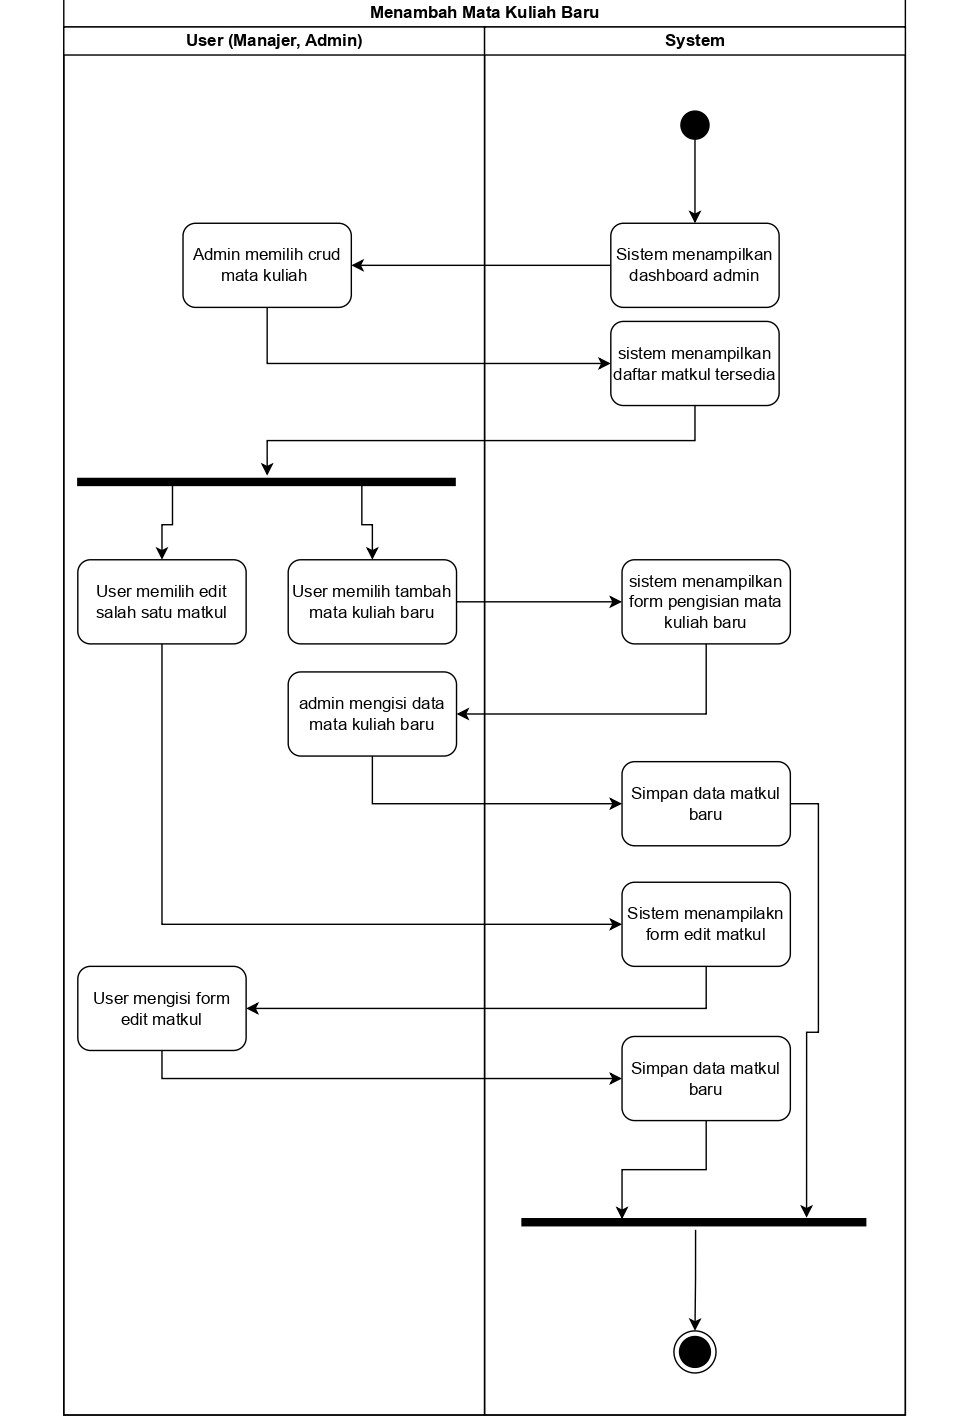
\includegraphics[width=0.8\textwidth]{Activity Diagram/Mata kuliah.jpg}
  \caption{Activity Diagram Mata Kuliah}
  \label{fig:activity_mata_kuliah}
\end{figure}
\subsubsection{Penjelasan Activity Diagram Mahasiswa Baru}
Activity Diagram Mahasiswa Baru pada Gambar~\ref{fig:activity_mahasiswa_baru} menggambarkan proses terstruktur penambahan data mahasiswa baru dalam sistem informasi akademik, dengan interaksi antara user (manajer dan admin) dan sistem. Diagram ini terdiri dari dua swimlane utama, yaitu swimlane untuk User (Manajer dan Admin) dan swimlane untuk System, yang memperjelas pembagian tugas dan alur kerja pada proses administrasi mahasiswa baru.

Langkah pertama dimulai dari sisi sistem, di mana sistem menampilkan dashboard admin sebagai antarmuka utama bagi user yang memiliki hak akses manajerial atau administratif. Dashboard ini berfungsi sebagai pusat kontrol untuk berbagai aktivitas administrasi, termasuk pengelolaan data mahasiswa. Setelah dashboard tampil, admin memilih menu CRUD mahasiswa baru, yang merupakan fitur untuk mengelola data mahasiswa secara komprehensif, mulai dari penambahan, pengeditan, hingga penghapusan data.

Setelah menu CRUD mahasiswa baru dipilih, sistem menampilkan daftar mahasiswa yang sudah tersedia di database. Tahap ini penting untuk memberikan gambaran kepada admin mengenai data mahasiswa yang telah ada, sehingga dapat menghindari duplikasi dan memudahkan monitoring data. Selanjutnya, admin memilih opsi tambah mahasiswa baru, yang menandai dimulainya proses input data mahasiswa baru ke dalam sistem.

Pada tahap berikutnya, sistem menampilkan form pengisian data mahasiswa baru. Form ini biasanya berisi berbagai field yang harus diisi oleh admin, seperti nama, NIM, email, program studi, dan data identitas lainnya yang relevan. Admin kemudian mengisi data mahasiswa baru secara lengkap dan akurat sesuai dengan persyaratan institusi. Proses pengisian data ini sangat krusial karena akan menentukan validitas dan integritas data mahasiswa di dalam sistem.

Setelah data mahasiswa baru diisi, admin mengirimkan data tersebut ke sistem dengan menekan tombol simpan. Sistem kemudian melakukan validasi terhadap data yang diinput, seperti pengecekan kelengkapan data, format email, dan ketersediaan NIM agar tidak terjadi duplikasi atau kesalahan input. Jika validasi berhasil, sistem akan menyimpan data mahasiswa baru ke dalam database dan memperbarui daftar mahasiswa yang tersedia. Jika terjadi error, seperti data duplikat atau format tidak sesuai, sistem akan menampilkan pesan peringatan agar admin dapat memperbaiki input sebelum data disimpan.

Diagram~\ref{fig:activity_mahasiswa_baru} juga menampilkan validasi hak akses, di mana hanya user dengan role admin atau manajer yang dapat melakukan penambahan mahasiswa baru. Validasi ini penting untuk menjaga keamanan dan integritas data, serta memastikan bahwa proses administrasi dilakukan oleh pihak yang berwenang. Setiap langkah dalam proses ini tercatat dengan baik, sehingga dapat digunakan sebagai referensi atau audit administrasi di kemudian hari.

Secara keseluruhan, Activity Diagram Mahasiswa Baru pada seperti pada Gambar~\ref{fig:activity_mahasiswa_baru} menunjukkan bagaimana sistem mendukung proses penambahan mahasiswa baru secara terstruktur, efisien, dan aman. Dengan adanya fitur ini, institusi pendidikan dapat memperbarui data mahasiswa secara berkala, menambah mahasiswa baru sesuai kebutuhan, dan menjaga kualitas data akademik. Proses yang digambarkan dalam diagram ini juga memastikan bahwa setiap langkah tercatat dengan baik, sehingga dapat digunakan sebagai referensi atau audit administrasi di kemudian hari. Fitur penambahan mahasiswa baru yang terintegrasi dalam sistem informasi akademik sangat penting untuk mendukung pengelolaan sumber daya manusia di lingkungan kampus. Dengan alur yang jelas, validasi data yang ketat, dan hak akses yang terjaga, sistem dapat meminimalisir risiko kesalahan input, menjaga keamanan data, serta meningkatkan efisiensi proses administrasi mahasiswa secara keseluruhan.

\subsection{Activity Diagram Mata Kuliah}
\begin{figure}[H]
  \centering
  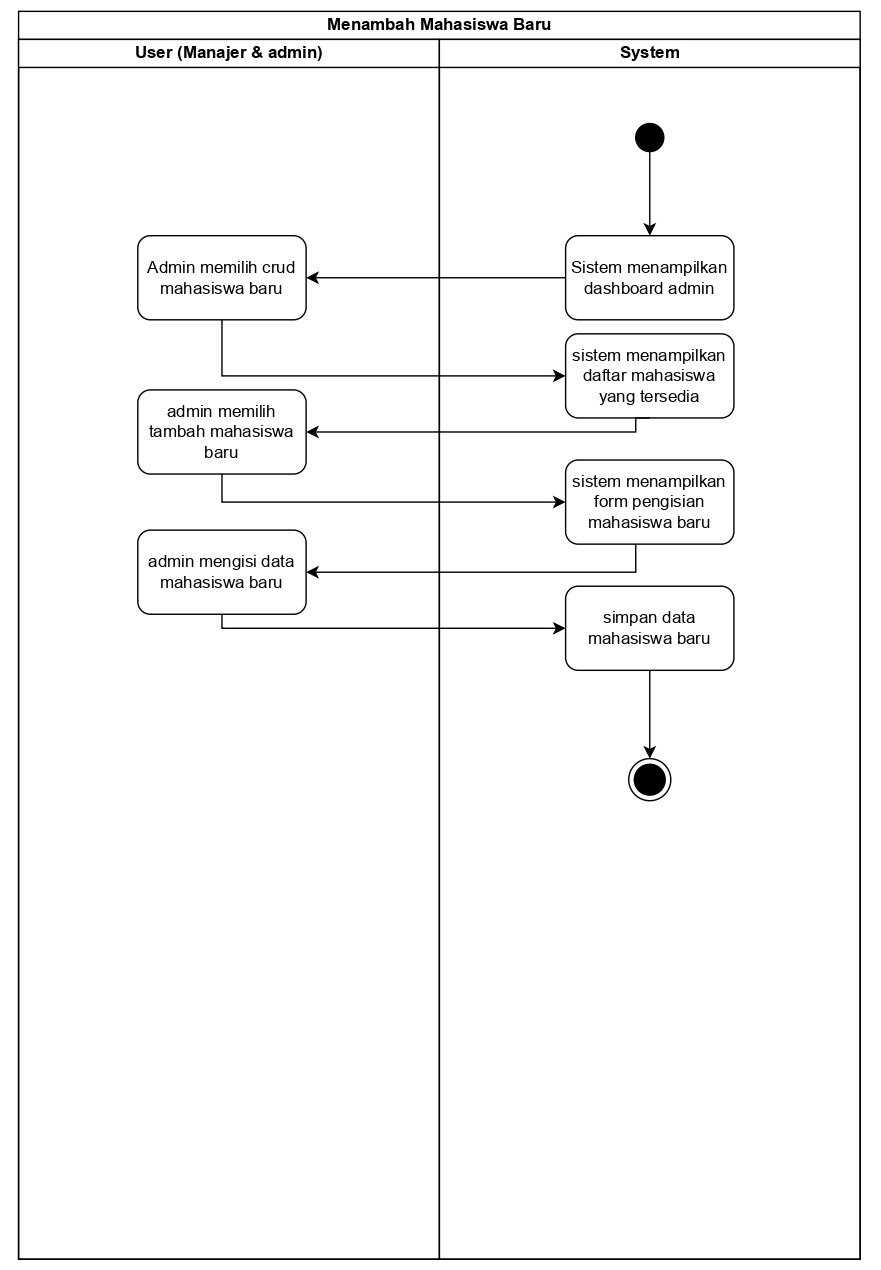
\includegraphics[width=0.8\textwidth]{Activity Diagram/Mahasiswa Baru.jpg}
  \caption{Activity Diagram Mahasiswa Baru}
  \label{fig:activity_mahasiswa_baru}
\end{figure}
\subsubsection{Penjelasan Activity Diagram Mata Kuliah}
Activity Diagram Mata Kuliah pada Gambar~\ref{fig:activity_mata_kuliah} menggambarkan proses penambahan dan pengelolaan data mata kuliah baru dalam sistem informasi akademik, dengan interaksi yang jelas antara user (manajer dan admin) dan sistem. Diagram ini terdiri dari dua swimlane utama, yaitu swimlane untuk User (Manajer, Admin) dan swimlane untuk System, yang memperjelas pembagian peran dan alur kerja pada proses administrasi mata kuliah.

Proses dimulai dari sisi sistem, di mana sistem menampilkan dashboard admin sebagai antarmuka utama bagi user yang memiliki hak akses administratif. Dashboard ini menjadi pusat kontrol untuk berbagai aktivitas, termasuk pengelolaan data mata kuliah. Setelah dashboard tampil, admin memilih menu CRUD mata kuliah, yang merupakan fitur untuk mengelola data mata kuliah secara menyeluruh, mulai dari penambahan, pengeditan, hingga penghapusan data.

Setelah menu CRUD mata kuliah dipilih, sistem menampilkan daftar mata kuliah yang sudah tersedia di database. Tahap ini penting untuk memberikan gambaran kepada admin mengenai data mata kuliah yang telah ada, sehingga dapat menghindari duplikasi dan memudahkan monitoring data. Pada titik ini, user dapat memilih dua jalur utama: menambah mata kuliah baru atau mengedit salah satu mata kuliah yang sudah ada.

Jika user memilih untuk menambah mata kuliah baru, sistem akan selanjutnya kemudian menampilkan form pengisian data mata kuliah baru. Form ini biasanya berisi field seperti nama mata kuliah, kode, jumlah SKS, dan deskripsi singkat. Admin kemudian mengisi data mata kuliah baru secara lengkap dan akurat. Setelah data diisi, admin mengirimkan data tersebut ke sistem dengan menekan tombol simpan. Sistem kemudian melakukan validasi terhadap data yang diinput, seperti pengecekan kelengkapan data dan ketersediaan kode mata kuliah agar tidak terjadi duplikasi. Jika validasi berhasil, sistem akan menyimpan data mata kuliah baru ke dalam database dan memperbarui daftar mata kuliah yang tersedia.

Jika user memilih untuk mengedit salah satu mata kuliah yang sudah ada, sistem akan menampilkan form edit mata kuliah. User kemudian mengisi form edit sesuai kebutuhan, misalnya memperbarui nama, jumlah SKS, atau deskripsi mata kuliah. Setelah form edit diisi, sistem kembali melakukan validasi dan menyimpan perubahan data ke dalam database.

Diagram~\ref{fig:activity_mata_kuliah} juga menampilkan validasi hak akses, di mana hanya user dengan role admin atau manajer yang dapat melakukan penambahan atau pengeditan data mata kuliah. Validasi ini penting untuk menjaga keamanan dan integritas data, serta memastikan bahwa proses administrasi dilakukan oleh pihak yang berwenang. Setiap langkah dalam proses ini tercatat dengan baik, sehingga dapat digunakan sebagai referensi atau audit administrasi di kemudian hari.

Secara keseluruhan, Activity Diagram Mata Kuliah pada Gambar~\ref{fig:activity_mata_kuliah} menunjukkan tentang bagaimana sistem mendukung proses penambahan dan pengelolaan data mata kuliah secara terstruktur, efisien, dan aman. Dengan adanya fitur ini, institusi pendidikan dapat memperbarui data mata kuliah secara berkala, menambah mata kuliah baru sesuai kebutuhan, dan menjaga kualitas data akademik. Proses yang digambarkan dalam diagram ini juga memastikan bahwa setiap langkah tercatat dengan baik, sehingga dapat digunakan sebagai referensi atau audit administrasi di kemudian hari. Fitur pengelolaan mata kuliah yang terintegrasi dalam sistem informasi akademik sangat penting untuk mendukung pengelolaan kurikulum dan proses pembelajaran di lingkungan kampus. Dengan alur yang jelas, validasi data yang ketat, dan hak akses yang terjaga, sistem dapat meminimalisir risiko kesalahan input, menjaga keamanan data, serta meningkatkan efisiensi proses administrasi mata kuliah secara keseluruhan.

\subsection{Activity Diagram Nilai Akhir}
\begin{figure}[H]
  \centering
  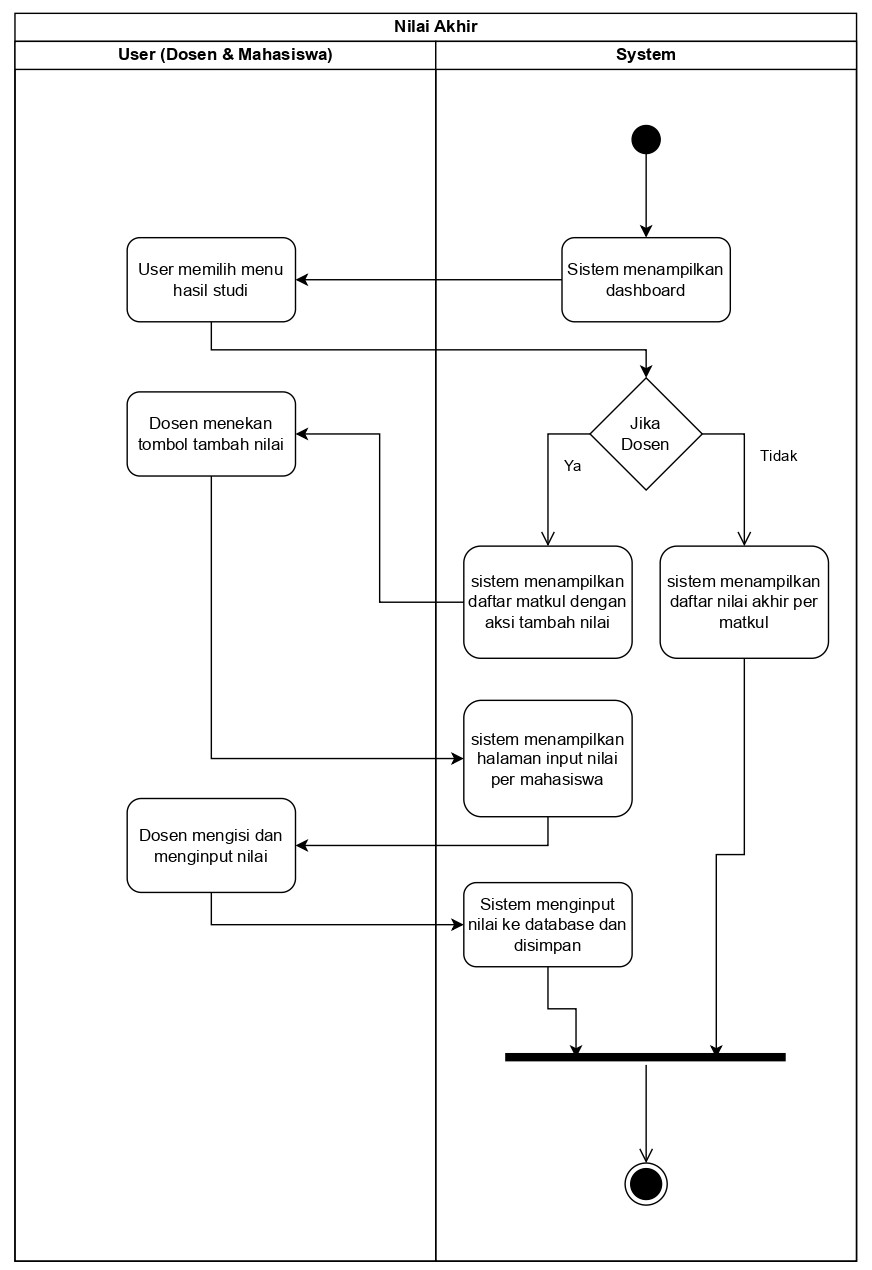
\includegraphics[width=0.8\textwidth]{Activity Diagram/Nilai Akhir.jpg}
  \caption{Activity Diagram Nilai Akhir}
  \label{fig:activity_nilai_akhir}
\end{figure}
\subsubsection{Penjelasan Activity Diagram Nilai Akhir}
Activity Diagram Nilai Akhir pada Gambar~\ref{fig:activity_nilai_akhir} menggambarkan proses pengelolaan dan input nilai akhir mahasiswa dalam sistem informasi akademik, dengan interaksi antara user (dosen dan mahasiswa) dan sistem. Diagram ini terdiri dari dua tugas utama, yaitu tugas untuk User (Dosen dan Mahasiswa) untuk System, yang memperjelas pembagian peran dan alur kerja pada proses penilaian akhir.

Proses dimulai ketika user memilih menu hasil studi pada dashboard aplikasi. Sistem kemudian menampilkan dashboard yang berisi berbagai fitur akademik, termasuk akses ke data nilai akhir. Pada tahap ini, sistem melakukan pengecekan role user. Jika user adalah dosen, sistem akan menampilkan daftar mata kuliah yang diampu beserta opsi untuk menambah nilai. Jika user adalah mahasiswa, sistem akan langsung menampilkan daftar nilai akhir per mata kuliah yang telah diambil.

Bagi dosen, langkah selanjutnya adalah menekan tombol tambah nilai pada salah satu mata kuliah yang diampu. Sistem kemudian menampilkan halaman input nilai per mahasiswa untuk mata kuliah tersebut. Pada halaman ini, dosen dapat mengisi dan menginput nilai akhir setiap mahasiswa secara individual. Proses input nilai ini sangat penting untuk memastikan bahwa data nilai yang dimasukkan akurat dan sesuai dengan hasil evaluasi pembelajaran.

Setelah dosen mengisi dan menginput nilai, sistem akan melakukan validasi terhadap data yang diinput, seperti pengecekan kelengkapan nilai dan format data. Jika validasi berhasil, sistem akan menginput nilai ke database dan menyimpan data tersebut secara permanen. Proses penyimpanan ini memastikan bahwa nilai akhir mahasiswa tercatat dengan baik dan dapat diakses oleh mahasiswa melalui menu hasil studi.

Bagi mahasiswa, sistem secara otomatis menampilkan daftar nilai akhir per mata kuliah yang telah diambil, sehingga mahasiswa dapat memantau perkembangan akademik mereka secara mandiri. Fitur ini juga memberikan transparansi dan kemudahan akses terhadap data nilai, sehingga mahasiswa dapat segera mengetahui hasil evaluasi pembelajaran tanpa harus menunggu pengumuman manual dari dosen.

Diagram~\ref{fig:activity_nilai_akhir} juga menampilkan validasi hak akses, di mana hanya dosen yang berwenang dapat melakukan input nilai, sedangkan mahasiswa hanya dapat melihat hasil nilai akhir. Validasi ini penting untuk menjaga keamanan dan integritas data, serta memastikan bahwa proses penilaian dilakukan oleh pihak yang berwenang. Setiap langkah dalam proses ini tercatat dengan baik, sehingga dapat digunakan sebagai referensi atau audit administrasi di kemudian hari.

Secara keseluruhan, Activity Diagram Nilai Akhir pada Gambar~\ref{fig:activity_nilai_akhir} menunjukkan tentang bagaimana sistem mendukung proses input dan pengelolaan nilai akhir secara terstruktur, efisien, dan aman. Dengan adanya fitur ini, institusi pendidikan dapat memperbarui data nilai secara berkala, memberikan akses transparan kepada mahasiswa, dan menjaga kualitas data akademik. Proses yang digambarkan dalam diagram ini juga memastikan bahwa setiap langkah tercatat dengan baik, sehingga dapat digunakan sebagai referensi atau audit administrasi di kemudian hari. Fitur pengelolaan nilai akhir yang terintegrasi dalam sistem informasi akademik sangat penting untuk mendukung evaluasi pembelajaran, transparansi, dan akuntabilitas di lingkungan kampus. Dengan alur yang jelas, validasi data yang ketat, dan hak akses yang terjaga, sistem dapat meminimalisir risiko kesalahan input, menjaga keamanan data, serta meningkatkan efisiensi proses administrasi nilai secara keseluruhan.


\subsection{Activity Diagram Pengumuman}
\begin{figure}[H]
  \centering
  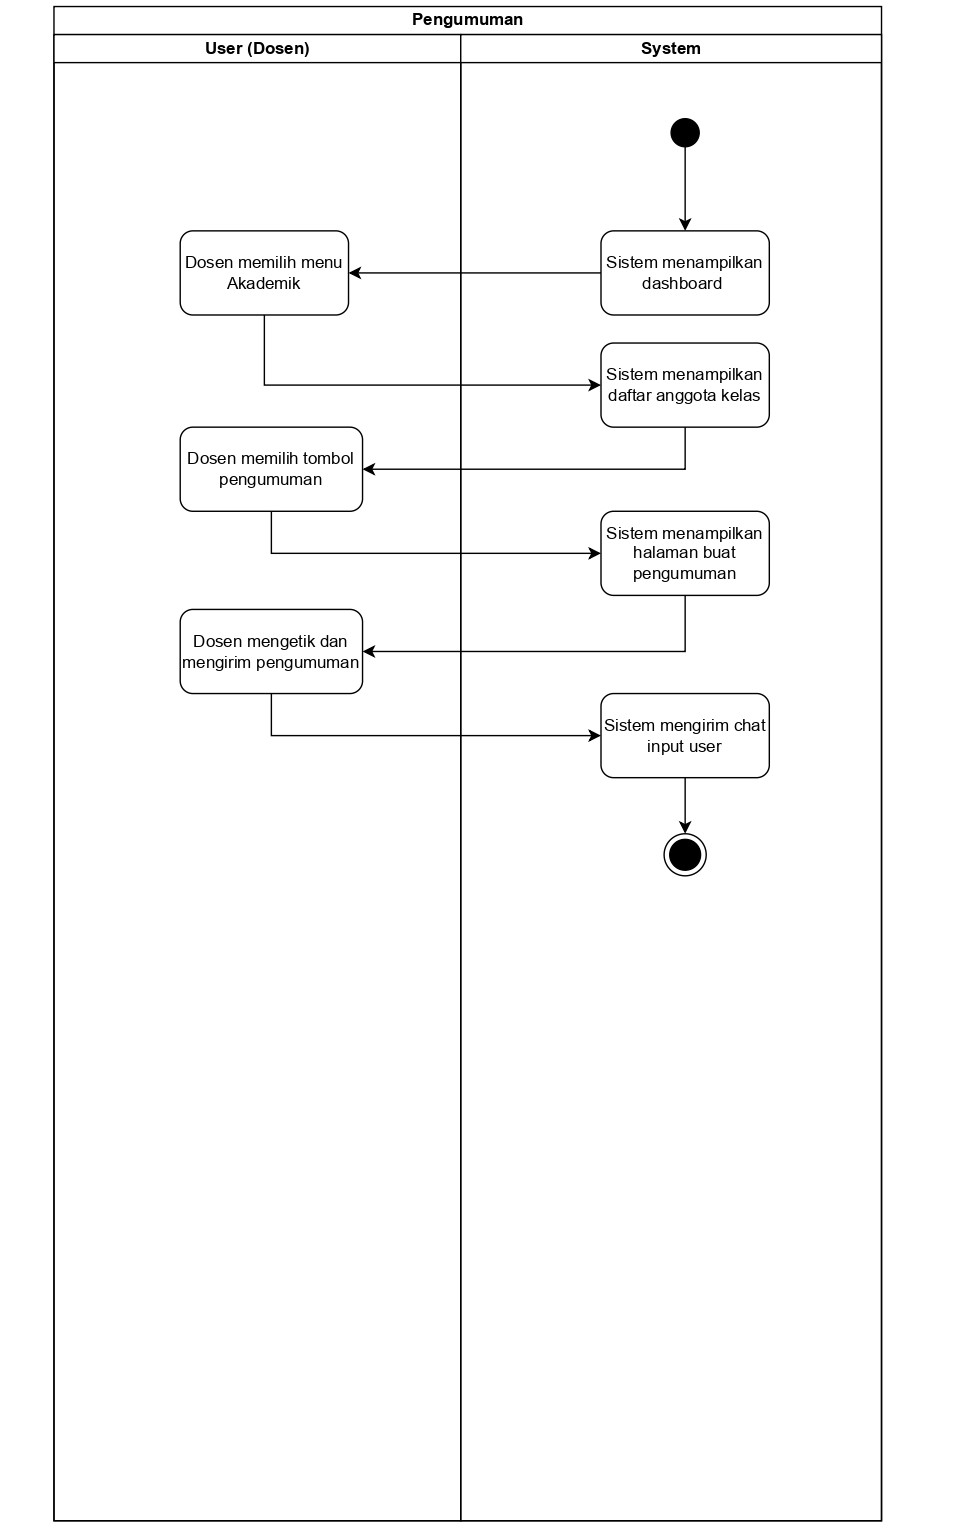
\includegraphics[width=0.8\textwidth]{Activity Diagram/Pengumuman.jpg}
  \caption{Activity Diagram Pengumuman}
  \label{fig:activity_pengumuman}
\end{figure}
\subsubsection{Penjelasan Activity Diagram Pengumuman}
Activity Diagram Pengumuman pada Gambar~\ref{fig:activity_pengumuman} menggambarkan proses pembuatan dan pengiriman pengumuman oleh dosen dalam sistem informasi akademik. Diagram ini terdiri dari dua swimlane utama, yaitu swimlane untuk User (Dosen) dan swimlane untuk System, yang memperjelas pembagian peran dan alur kerja pada proses penyampaian pengumuman kepada anggota kelas.

Proses dimulai ketika dosen memilih menu Akademik pada dashboard aplikasi. Sistem merespons dengan menampilkan dashboard utama yang berisi berbagai fitur akademik, termasuk daftar anggota kelas yang menjadi target pengumuman. Tahap ini penting untuk memastikan dosen dapat memilih kelas atau kelompok yang relevan sebelum membuat pengumuman.

Setelah dashboard dan daftar anggota kelas ditampilkan, dosen memilih tombol pengumuman untuk memulai proses pembuatan pengumuman baru. Sistem kemudian menampilkan halaman khusus untuk membuat pengumuman, di mana dosen dapat mengetik isi pengumuman yang ingin disampaikan kepada mahasiswa atau anggota kelas lainnya. Halaman ini biasanya dilengkapi dengan fitur untuk memilih target penerima, mengatur format pesan, dan menambahkan lampiran jika diperlukan.

Setelah dosen selesai mengetik dan mengirim pengumuman, sistem akan memproses input tersebut dan mengirimkan pengumuman ke seluruh anggota kelas yang dituju. Pengiriman pengumuman dapat dilakukan melalui berbagai kanal, seperti notifikasi aplikasi, email, atau chat internal sistem, tergantung pada pengaturan dan preferensi institusi. Sistem juga dapat mencatat waktu pengiriman dan status penerimaan pengumuman untuk keperluan monitoring dan audit.

Diagram~\ref{fig:activity_pengumuman} menekankan pentingnya validasi hak akses, di mana hanya dosen yang berwenang dapat membuat dan mengirim pengumuman kepada kelas. Validasi ini penting untuk menjaga keamanan informasi dan memastikan bahwa hanya informasi resmi yang disampaikan kepada mahasiswa. Setiap langkah dalam proses ini tercatat dengan baik, sehingga dapat digunakan sebagai referensi atau audit administrasi di kemudian hari.

Secara keseluruhan, Activity Diagram Pengumuman pada Gambar~\ref{fig:activity_pengumuman} menunjukkan bagaimana sistem mendukung proses pembuatan dan pengiriman pengumuman secara terstruktur, efisien, dan aman. Dengan adanya fitur ini, dosen dapat menyampaikan informasi penting, jadwal, atau perubahan kebijakan kepada mahasiswa secara cepat dan terorganisir. Proses yang digambarkan dalam diagram ini juga memastikan bahwa setiap pengumuman tercatat dan dapat diakses kembali jika diperlukan. Fitur pengumuman yang terintegrasi dalam sistem informasi akademik sangat penting untuk mendukung komunikasi akademik, meningkatkan transparansi, dan mempercepat penyebaran informasi di lingkungan kampus. Dengan alur yang jelas, validasi data yang ketat, dan hak akses yang terjaga, sistem dapat meminimalisir risiko miskomunikasi, menjaga keamanan data, serta meningkatkan efisiensi proses komunikasi akademik secara keseluruhan.


\subsection{Activity Diagram Presensi}
\begin{figure}[H]
  \centering
  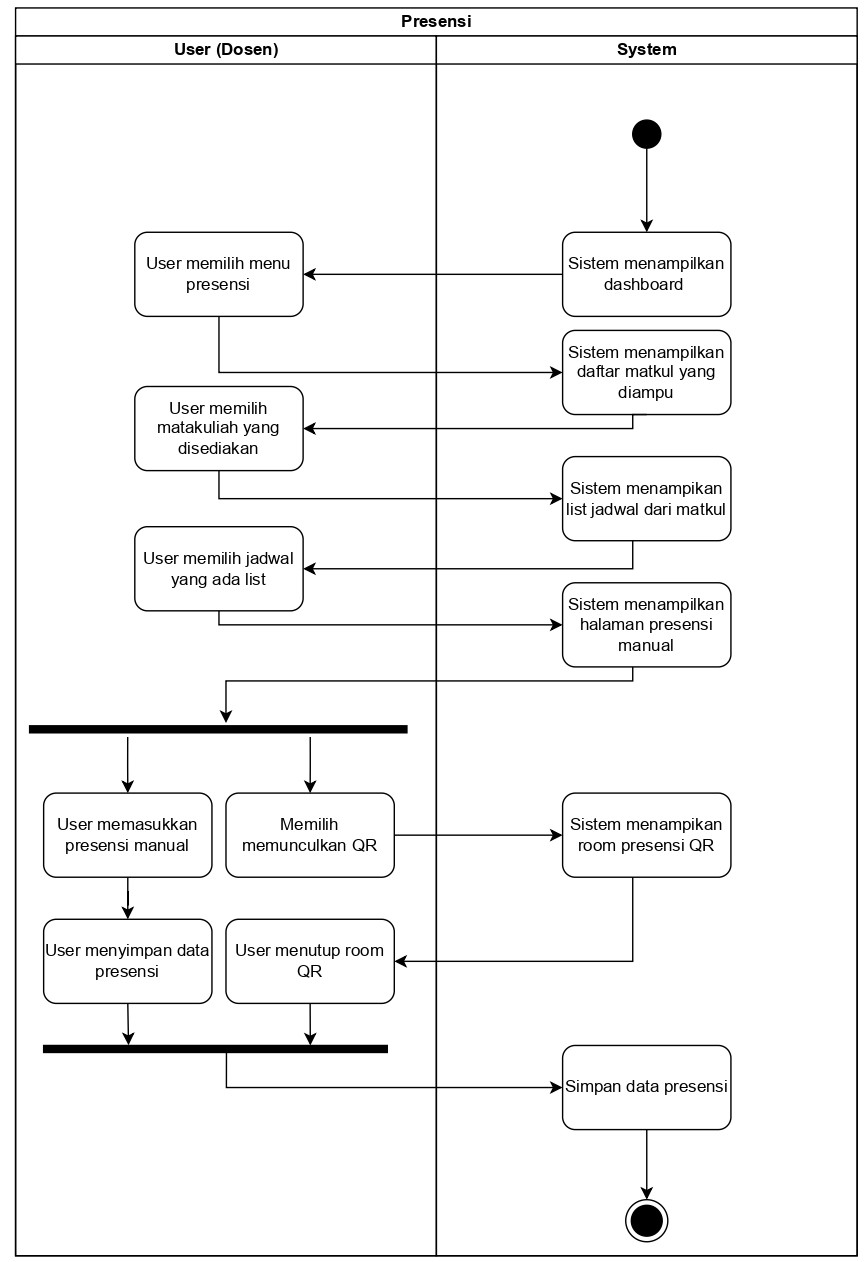
\includegraphics[width=0.8\textwidth]{Activity Diagram/Presensi.jpg}
  \caption{Activity Diagram Presensi}
  \label{fig:activity_presensi}
\end{figure}
\subsubsection{Penjelasan Activity Diagram Presensi}
Activity Diagram Presensi pada Gambar~\ref{fig:activity_presensi} menggambarkan proses pencatatan kehadiran mahasiswa yang dilakukan oleh dosen dalam sistem informasi akademik. Diagram ini terdiri dari dua swimlane utama, yaitu swimlane untuk User (Dosen) dan swimlane untuk System, yang memperjelas pembagian peran dan alur kerja pada proses presensi.

Proses dimulai ketika dosen memilih menu presensi pada dashboard aplikasi. Sistem kemudian menampilkan dashboard utama yang berisi daftar mata kuliah yang diampu oleh dosen. Tahap ini penting untuk memastikan dosen hanya dapat mengakses dan mengelola presensi pada mata kuliah yang menjadi tanggung jawabnya.

Setelah daftar mata kuliah ditampilkan, dosen memilih salah satu mata kuliah yang tersedia. Sistem kemudian menampilkan list jadwal dari mata kuliah tersebut, sehingga dosen dapat memilih jadwal perkuliahan yang sesuai dengan waktu pelaksanaan presensi. Setelah jadwal dipilih, sistem menampilkan halaman presensi manual yang berisi opsi untuk melakukan presensi secara manual atau menggunakan QR code.

Pada tahap ini, dosen dapat memilih dua jalur utama: memasukkan presensi manual atau memilih untuk memunculkan QR. Jika dosen memilih presensi manual, dosen akan menginput data kehadiran mahasiswa secara langsung pada halaman yang disediakan. Setelah data presensi diisi, dosen menyimpan data presensi tersebut ke dalam sistem. Jika dosen memilih untuk memunculkan QR, sistem akan menampilkan room presensi QR yang dapat diakses oleh mahasiswa untuk melakukan presensi secara digital. Setelah proses presensi QR selesai, dosen dapat menutup room QR.

Setelah salah satu metode presensi selesai dilakukan, sistem akan menyimpan data presensi ke dalam database. Proses penyimpanan ini memastikan bahwa data kehadiran mahasiswa tercatat dengan baik dan dapat diakses untuk keperluan monitoring, rekapitulasi, atau audit di kemudian hari.

Diagram~\ref{fig:activity_presensi} juga menampilkan validasi hak akses, di mana hanya dosen yang berwenang dapat mengelola presensi pada mata kuliah yang diampu. Validasi ini penting untuk menjaga keamanan dan integritas data kehadiran, serta memastikan bahwa proses presensi dilakukan oleh pihak yang berwenang. Setiap langkah dalam proses ini tercatat dengan baik, sehingga dapat digunakan sebagai referensi atau audit administrasi di kemudian hari.

Secara keseluruhan, Activity Diagram Presensi pada Gambar~\ref{fig:activity_presensi} menunjukkan bagaimana sistem mendukung proses pencatatan kehadiran mahasiswa secara terstruktur, efisien, dan aman. Dengan adanya fitur presensi manual dan QR, institusi pendidikan dapat menyesuaikan metode presensi sesuai kebutuhan, meningkatkan akurasi data kehadiran, dan memudahkan monitoring kehadiran mahasiswa. Proses yang digambarkan dalam diagram ini juga memastikan bahwa setiap langkah tercatat dengan baik, sehingga dapat digunakan sebagai referensi atau audit administrasi di kemudian hari. Fitur presensi yang terintegrasi dalam sistem informasi akademik sangat penting untuk mendukung pengelolaan kehadiran, meningkatkan disiplin, dan memperkuat akuntabilitas di lingkungan kampus. Dengan alur yang jelas, validasi data yang ketat, dan hak akses yang terjaga, sistem dapat meminimalisir risiko kesalahan input, menjaga keamanan data, serta meningkatkan efisiensi proses administrasi presensi secara keseluruhan.


\subsection{Activity Diagram Scan Presensi}
\begin{figure}[H]
  \centering
  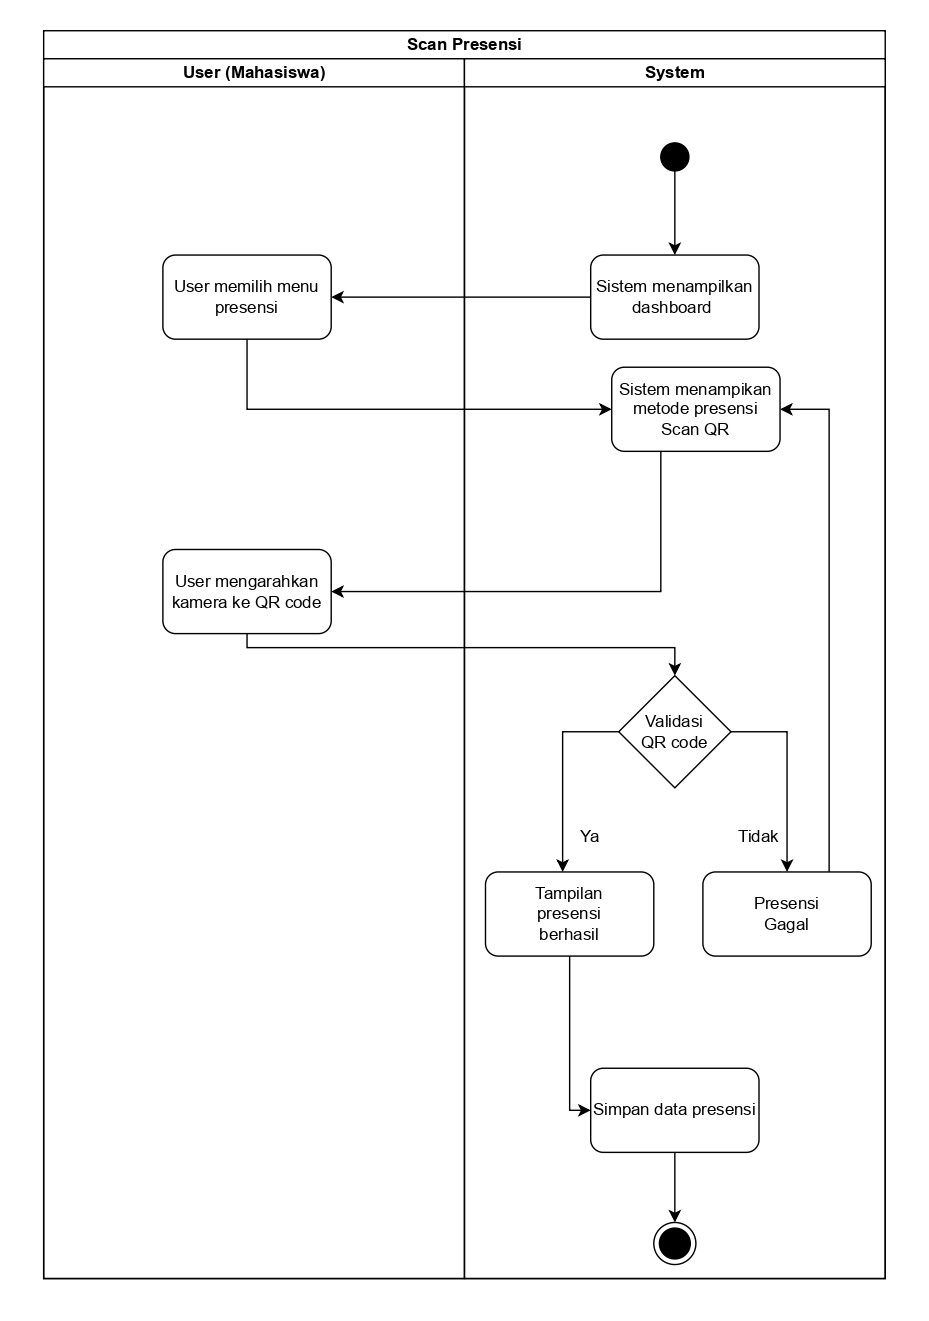
\includegraphics[width=0.8\textwidth]{Activity Diagram/Scan Presensi.jpg}
  \caption{Activity Diagram Scan Presensi}
  \label{fig:activity_scan_presensi}
\end{figure}

\subsubsection{Penjelasan Activity Diagram Scan Presensi}
Activity Diagram Scan Presensi pada Gambar~\ref{fig:activity_scan_presensi} menggambarkan proses presensi mahasiswa menggunakan metode pemindaian QR code pada sistem informasi akademik. Diagram ini terdiri dari dua swimlane utama, yaitu User (Mahasiswa) dan System, yang memperjelas pembagian peran antara pengguna dan sistem selama proses presensi berlangsung.

Proses dimulai dari sisi sistem, di mana sistem menampilkan dashboard utama setelah user berhasil login. Dashboard ini berfungsi sebagai pusat navigasi bagi mahasiswa untuk mengakses berbagai fitur, salah satunya menu presensi. Ketika mahasiswa memilih menu presensi, sistem akan menampilkan pilihan metode presensi, dalam hal ini adalah Scan QR. Sistem kemudian menampilkan instruksi atau tampilan untuk melakukan pemindaian QR code.

Selanjutnya, mahasiswa mengarahkan kamera perangkat ke QR code yang telah disediakan oleh dosen atau sistem di ruang kelas. Proses ini merupakan interaksi langsung antara user dan sistem, di mana sistem akan melakukan pemindaian dan validasi terhadap QR code yang diterima. Validasi QR code menjadi tahap krusial untuk memastikan bahwa QR code yang dipindai adalah valid, sesuai jadwal, dan belum pernah digunakan sebelumnya oleh user yang sama.

Jika validasi QR code berhasil, sistem akan menampilkan notifikasi atau tampilan bahwa presensi berhasil dilakukan. Pada tahap ini, data presensi mahasiswa akan disimpan ke dalam database sistem sebagai bukti kehadiran pada sesi tersebut. Proses penyimpanan data ini penting untuk memastikan integritas dan akurasi data kehadiran mahasiswa, yang nantinya dapat digunakan untuk rekapitulasi kehadiran, monitoring, maupun kebutuhan administrasi lainnya.

Sebaliknya, jika validasi QR code gagal—misalnya karena QR code tidak valid, sudah digunakan, atau terjadi kesalahan teknis—sistem akan menampilkan pesan presensi gagal. Mahasiswa dapat mencoba kembali atau meminta bantuan kepada petugas jika mengalami kendala. Sistem kemudian akan kembali ke tampilan metode presensi, memungkinkan user untuk mengulangi proses jika diperlukan.

Diagram \ref{fig:activity_scan_presensi} ini menekankan pentingnya validasi otomatis oleh sistem untuk mencegah kecurangan dan memastikan hanya mahasiswa yang hadir secara fisik yang dapat melakukan presensi. Selain itu, penggunaan QR code mempercepat proses presensi, mengurangi antrean, dan meminimalisir kontak fisik, sehingga sangat relevan untuk diterapkan dalam situasi pembelajaran modern, termasuk pembelajaran tatap muka terbatas.

Secara keseluruhan, Activity Diagram Scan Presensi \ref{fig:activity_scan_presensi} menunjukkan alur yang efisien, aman, dan terstruktur dalam proses pencatatan kehadiran mahasiswa. Dengan pembagian peran yang jelas antara user dan sistem, serta adanya validasi otomatis, sistem presensi berbasis QR code ini dapat meningkatkan akurasi data kehadiran, memudahkan monitoring, dan mendukung transparansi dalam pengelolaan kehadiran di lingkungan akademik.


\subsection{Activity Diagram Tambah Akun Manajer}
\begin{figure}[H]
  \centering
  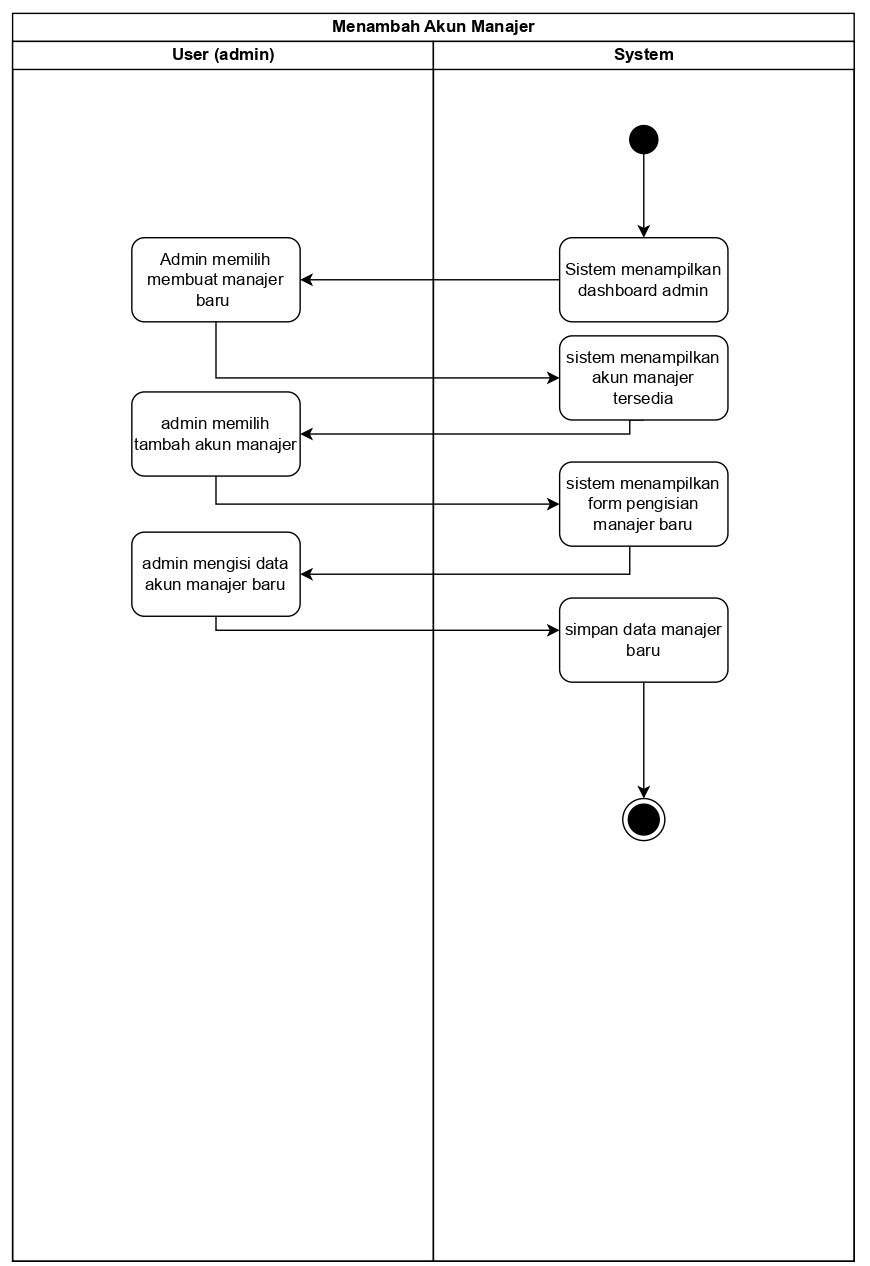
\includegraphics[width=0.8\textwidth]{Activity Diagram/Tambah akun manajer.jpg}
  \caption{Activity Diagram Tambah Akun Manajer}
  \label{fig:activity_tambah_akun_manajer}
\end{figure}

\subsubsection{Penjelasan Activity Diagram Tambah Akun Manajer}
Activity Diagram Tambah Akun Manajer pada Gambar~\ref{fig:activity_tambah_akun_manajer} menggambarkan proses penambahan akun manajer baru oleh admin dalam sistem informasi akademik. Diagram ini terdiri dari dua swimlane utama, yaitu User (admin) dan System, yang memperjelas pembagian peran dan alur kerja antara admin sebagai pengguna dan sistem sebagai penyedia layanan.

Proses dimulai dari sisi sistem, di mana sistem menampilkan dashboard admin sebagai antarmuka utama setelah admin berhasil login. Dashboard ini berfungsi sebagai pusat kontrol bagi admin untuk mengelola berbagai fitur, salah satunya adalah pengelolaan akun manajer. Ketika admin memilih menu untuk membuat manajer baru, sistem akan menampilkan daftar akun manajer yang sudah tersedia. Tahap ini penting untuk memberikan gambaran kepada admin mengenai data manajer yang telah ada, sehingga dapat menghindari duplikasi dan memudahkan monitoring data.

Selanjutnya, admin memilih opsi tambah akun manajer. Sistem kemudian menampilkan form pengisian data manajer baru yang harus diisi oleh admin. Form ini biasanya berisi data identitas manajer seperti nama, email, username, dan informasi lain yang relevan. Pada tahap ini, admin mengisi data akun manajer baru secara lengkap dan akurat sesuai dengan kebutuhan institusi.

Setelah data akun manajer baru diisi, admin mengirimkan data tersebut ke sistem. Sistem kemudian melakukan proses penyimpanan data manajer baru ke dalam database. Proses penyimpanan ini sangat penting untuk memastikan bahwa data manajer baru tercatat dengan baik dan dapat digunakan untuk keperluan administrasi selanjutnya. Jika terjadi error, seperti data duplikat atau format tidak sesuai, sistem akan menampilkan pesan peringatan agar admin dapat memperbaiki input sebelum data disimpan.

Diagram~\ref{fig:activity_tambah_akun_manajer} ini menekankan pentingnya validasi data dan kemudahan proses penambahan akun manajer oleh admin. Dengan adanya fitur ini, institusi pendidikan dapat memperbarui data manajer secara berkala, menambah manajer baru sesuai kebutuhan, dan menjaga kualitas data administrasi. Proses yang digambarkan dalam diagram ini juga memastikan bahwa setiap langkah tercatat dengan baik, sehingga dapat digunakan sebagai referensi atau audit administrasi di kemudian hari.

Secara keseluruhan, Activity Diagram Tambah Akun Manajer pada Gambar~\ref{fig:activity_tambah_akun_manajer} menunjukkan bagaimana sistem mendukung proses penambahan akun manajer secara terstruktur, efisien, dan aman. Dengan pembagian peran yang jelas antara admin dan sistem, serta adanya validasi data, sistem dapat meminimalisir risiko kesalahan input, menjaga keamanan data, serta meningkatkan efisiensi proses administrasi akun manajer di lingkungan kampus.


\subsection{Activity Diagram User Manajemen}
\begin{figure}[H]
  \centering
  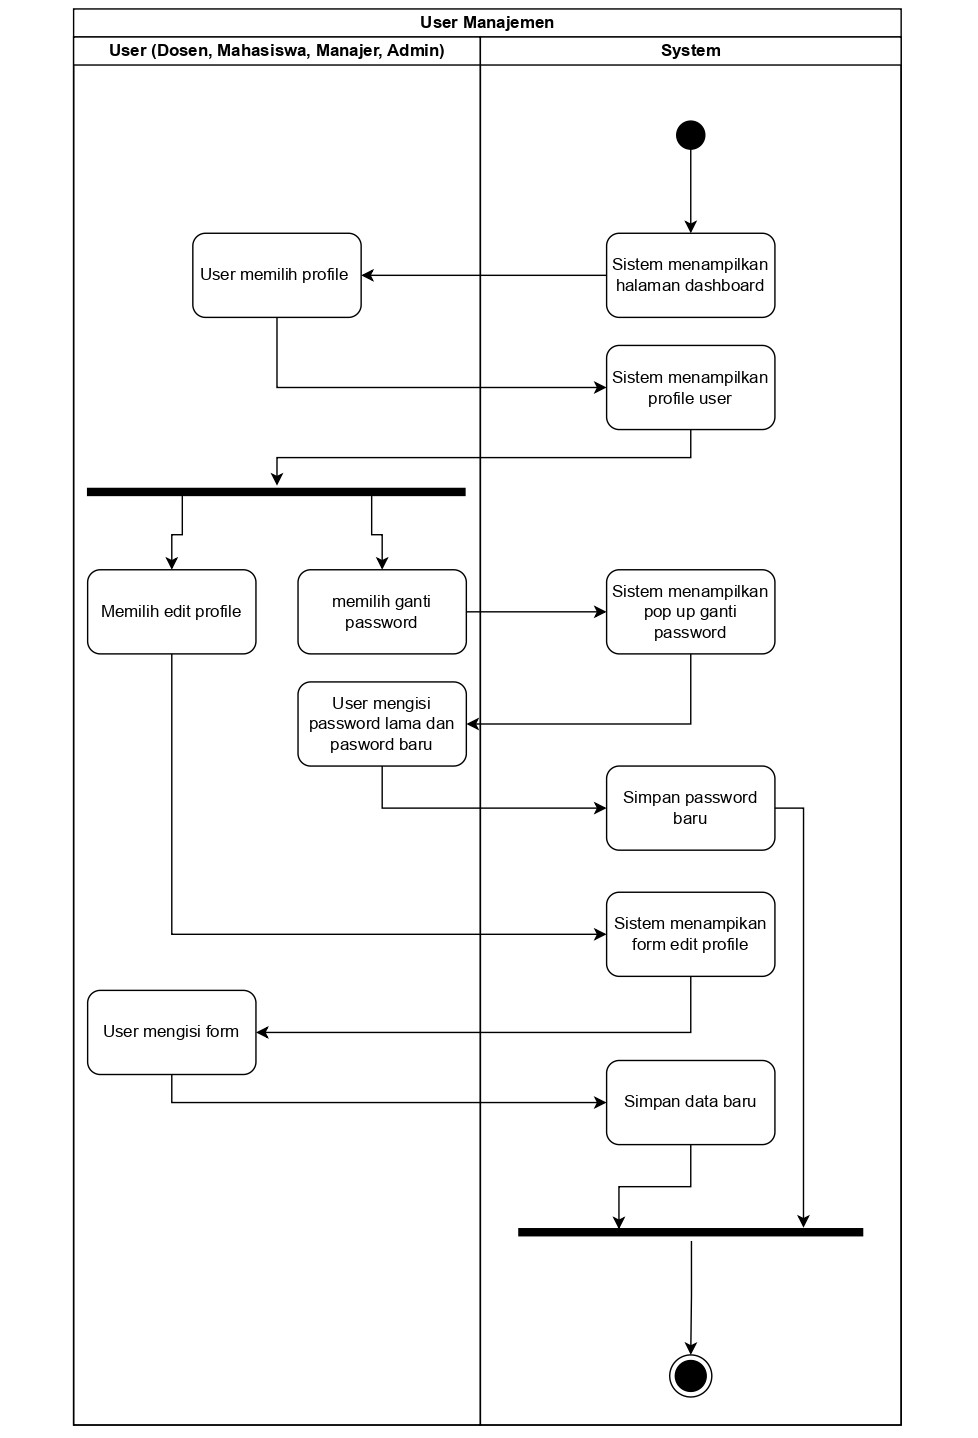
\includegraphics[width=0.8\textwidth]{Activity Diagram/User Manajemen.jpg}
  \caption{Activity Diagram User Manajemen}
  \label{fig:activity_user_manajemen}
\end{figure}

\subsubsection{Penjelasan Activity Diagram User Manajemen}
Activity Diagram User Manajemen pada Gambar~\ref{fig:activity_user_manajemen} menggambarkan proses pengelolaan data pengguna (user) dalam sistem informasi akademik, yang dapat dilakukan oleh berbagai peran seperti dosen, mahasiswa, manajer, maupun admin. Diagram ini terdiri dari dua swimlane utama, yaitu User (Dosen, Mahasiswa, Manajer, Admin) dan System, yang memperjelas pembagian peran antara pengguna dan sistem selama proses manajemen akun berlangsung.

Proses dimulai dari sisi sistem, di mana sistem menampilkan halaman dashboard setelah user berhasil login. Dashboard ini menjadi pusat navigasi bagi user untuk mengakses berbagai fitur, salah satunya adalah menu profile. Ketika user memilih menu profile, sistem akan menampilkan halaman profile user yang berisi informasi data diri dan pengaturan akun.

Selanjutnya, user dapat memilih dua jalur utama, yaitu edit profile atau ganti password. Jika user memilih edit profile, sistem akan menampilkan form edit profile yang dapat diisi untuk memperbarui data diri seperti nama, email, atau informasi lain yang relevan. Setelah form diisi, user mengirimkan data baru ke sistem, dan sistem akan menyimpan data baru tersebut ke dalam database. Proses ini memastikan bahwa data user selalu terupdate dan akurat.

Jika user memilih ganti password, sistem akan menampilkan pop up ganti password. User kemudian mengisi password lama dan password baru pada form yang disediakan. Setelah data diinput, sistem akan melakukan validasi dan menyimpan password baru ke dalam database. Proses ini penting untuk menjaga keamanan akun user dan memastikan hanya user yang berwenang yang dapat mengubah password.

Diagram~\ref{fig:activity_user_manajemen} ini menekankan pentingnya validasi data dan keamanan dalam proses manajemen akun. Setiap perubahan data, baik profile maupun password, harus melalui proses validasi oleh sistem untuk mencegah kesalahan input dan menjaga integritas data. Selain itu, sistem juga memastikan bahwa hanya user yang berhak yang dapat melakukan perubahan pada akun masing-masing.

Secara keseluruhan, Activity Diagram User Manajemen pada Gambar~\ref{fig:activity_user_manajemen} menunjukkan bagaimana sistem mendukung proses pengelolaan akun user secara terstruktur, efisien, dan aman. Dengan pembagian peran yang jelas antara user dan sistem, serta adanya validasi data dan keamanan, sistem dapat meminimalisir risiko kesalahan input, menjaga keamanan data, serta meningkatkan efisiensi proses administrasi akun di lingkungan kampus.

\section{ERD}
\begin{figure}[H]
  \centering
  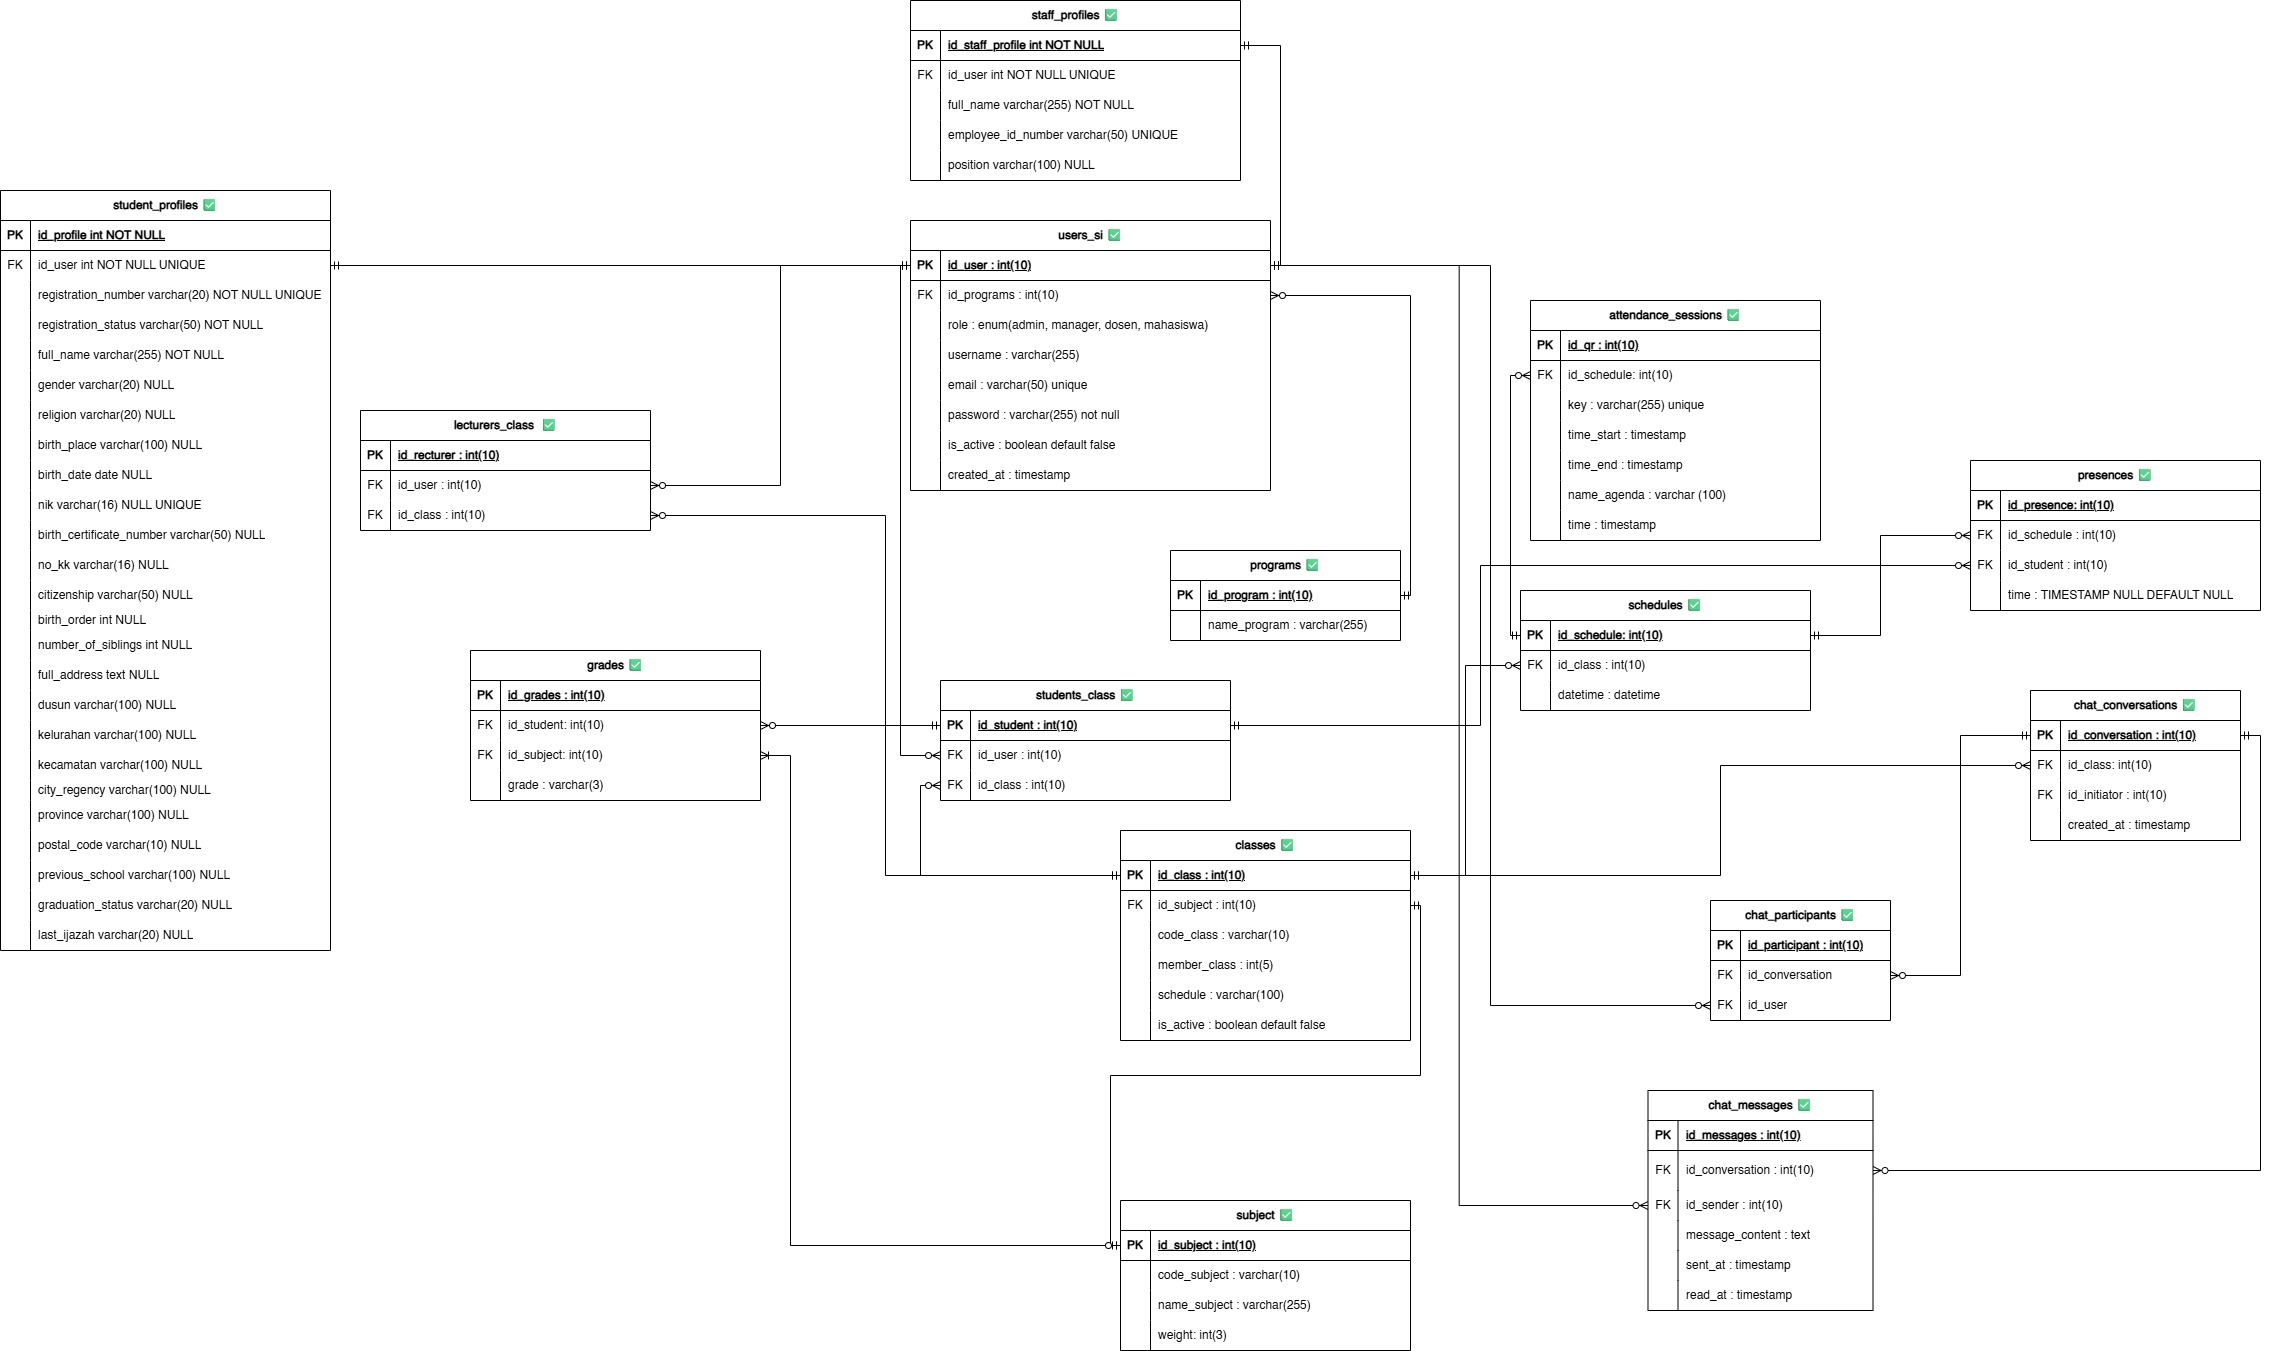
\includegraphics[width=0.8\textwidth]{ERD/SIAKampus-ERD.jpg}
  \caption{ERD Sistem Informasi Akademik}
  \label{fig:erd_sistem_informasi_akademik}
\end{figure}

\subsubsection{Penjelasan ERD Sistem Informasi Akademik}

Entity Relationship Diagram (ERD) pada Gambar~\ref{fig:erd_sistem_informasi_akademik} menggambarkan struktur basis data yang digunakan dalam Sistem Informasi Akademik (SIA) kampus. ERD ini terdiri dari berbagai entitas yang saling terhubung dan merepresentasikan proses-proses utama dalam pengelolaan data akademik, mulai dari manajemen pengguna, kelas, jadwal, presensi, nilai, hingga komunikasi antar civitas akademika. Berikut penjelasan detail setiap entitas, relasi, dan alur data yang terjadi dalam sistem.

\subsubsection{Aktor dan Peran}
\begin{itemize}
  \item \textbf{Mahasiswa}: Memiliki data profil, mengikuti kelas, melakukan presensi, menerima nilai, dan berkomunikasi melalui fitur chat.
  \item \textbf{Dosen}: Memiliki data profil, mengampu kelas, menginput nilai, membuat sesi presensi, dan berkomunikasi dengan mahasiswa.
  \item \textbf{Admin/Manager}: Mengelola data pengguna, program studi, kelas, dan monitoring seluruh aktivitas akademik.
\end{itemize}

\subsubsection{Tabel dan Entitas}
\begin{enumerate}
  \item \textbf{users\_si}: Menyimpan data seluruh pengguna (admin, manager, dosen, mahasiswa) beserta atribut identitas dan autentikasi.
  \item \textbf{student\_profiles} dan \textbf{staff\_profiles}: Menyimpan data detail profil mahasiswa dan staf/dosen.
  \item \textbf{programs}: Menyimpan daftar program studi yang diikuti oleh user.
  \item \textbf{classes}: Menyimpan data kelas, kode, jadwal, dan status aktif.
  \item \textbf{subject}: Menyimpan data mata kuliah, kode, nama, dan bobot SKS.
  \item \textbf{students\_class} dan \textbf{lecturers\_class}: Tabel penghubung antara mahasiswa/dosen dengan kelas yang diikuti/diampu.
  \item \textbf{grades}: Menyimpan nilai mahasiswa untuk setiap mata kuliah di kelas tertentu.
  \item \textbf{schedules}: Menyimpan jadwal perkuliahan, waktu mulai, selesai, dan agenda.
  \item \textbf{attendance\_sessions}: Menyimpan sesi presensi pada setiap jadwal kelas.
  \item \textbf{presences}: Menyimpan data kehadiran mahasiswa pada setiap sesi presensi.
  \item \textbf{chat\_conversations}, \textbf{chat\_participants}, \textbf{chat\_messages}: Menyimpan data percakapan, peserta, dan pesan dalam komunikasi kelas.
\end{enumerate}

\subsubsection{Relasi Antar Entitas}
\begin{itemize}
  \item \textbf{users\_si} terhubung ke \textbf{student\_profiles}, \textbf{staff\_profiles}, dan \textbf{programs}. Relasi ini berfungsi untuk mengelola data identitas, peran, dan program studi setiap pengguna. Dengan adanya relasi ini, sistem dapat membedakan antara mahasiswa, dosen, dan staf, serta mengaitkan mereka dengan program studi yang relevan.
  \item \textbf{users\_si} terhubung ke \textbf{students\_class} dan \textbf{lecturers\_class}. Relasi ini memungkinkan sistem mencatat kelas mana saja yang diikuti oleh mahasiswa dan diampu oleh dosen. Dengan demikian, sistem dapat mengelola daftar peserta dan pengajar setiap kelas secara dinamis.
  \item \textbf{classes} terhubung ke \textbf{students\_class}, yaitu untuk mencatat mahasiswa mana saja yang mengikuti kelas tersebut. Relasi ini memungkinkan sistem untuk mengelola daftar peserta kelas, absensi, dan nilai mahasiswa secara spesifik pada setiap kelas.
  \item \textbf{classes} terhubung ke \textbf{lecturers\_class}, yaitu untuk mencatat dosen mana saja yang mengampu atau bertanggung jawab atas kelas tersebut. Relasi ini penting untuk penjadwalan, penginputan nilai, dan monitoring aktivitas dosen dalam kelas.
  \item \textbf{classes} terhubung ke \textbf{schedules}, yaitu untuk mengatur jadwal perkuliahan yang terkait dengan kelas tersebut. Dengan relasi ini, setiap kelas dapat memiliki satu atau lebih jadwal yang mengatur waktu pelaksanaan perkuliahan, presensi, dan agenda akademik.
  \item \textbf{classes} terhubung ke \textbf{chat\_conversations}, yaitu untuk memfasilitasi komunikasi dan diskusi antara dosen dan mahasiswa dalam kelas. Relasi ini memungkinkan terciptanya ruang percakapan khusus untuk setiap kelas, sehingga informasi, pengumuman, dan diskusi dapat terdokumentasi dengan baik.
  \item \textbf{subject} terhubung ke \textbf{grades}. Relasi ini digunakan untuk mengelola proses input dan penyimpanan nilai mahasiswa berdasarkan mata kuliah yang diambil. Setiap nilai yang diinput dosen akan dikaitkan dengan mata kuliah tertentu.
  \item \textbf{schedules} terhubung ke \textbf{attendance\_sessions}. Relasi ini berfungsi untuk mengatur sesi presensi pada setiap jadwal perkuliahan. Dengan relasi ini, sistem dapat mencatat kehadiran mahasiswa dan dosen pada waktu yang telah dijadwalkan.
  \item \textbf{attendance\_sessions} terhubung ke \textbf{presences}. Relasi ini digunakan untuk mencatat kehadiran mahasiswa pada setiap sesi presensi yang telah dibuat. Data ini penting untuk monitoring absensi dan rekap kehadiran mahasiswa.
  \item \textbf{chat\_conversations} terhubung ke \textbf{chat\_participants} dan \textbf{chat\_messages}. Relasi ini memfasilitasi komunikasi dan diskusi antara dosen dan mahasiswa dalam kelas. Setiap percakapan akan memiliki daftar peserta dan kumpulan pesan yang terdokumentasi dengan baik.
\end{itemize}

\subsubsection{Alur Data dan Proses Akademik}
\begin{enumerate}
  \item \textbf{Pendaftaran dan Pengelolaan Akun}: Proses ini dimulai ketika user (mahasiswa, dosen, atau staf) melakukan pendaftaran di sistem. Data identitas dan autentikasi user disimpan di \textbf{users\_si}, kemudian dihubungkan ke \textbf{student\_profiles} atau \textbf{staff\_profiles} sesuai peran, serta dikaitkan dengan program studi di \textbf{programs}. Relasi ini memastikan setiap user memiliki profil lengkap dan terintegrasi dengan struktur akademik kampus.
  \item \textbf{Pengelolaan Kelas dan Jadwal}: Mahasiswa dan dosen dihubungkan ke kelas melalui tabel penghubung \textbf{students\_class} dan \textbf{lecturers\_class}. Setiap kelas memiliki jadwal yang diatur di \textbf{schedules}, sehingga sistem dapat mengelola waktu perkuliahan, pembagian kelas, dan penugasan dosen secara efisien.
  \item \textbf{Presensi dan Monitoring Kehadiran}: Pada setiap jadwal perkuliahan, dosen membuat sesi presensi di \textbf{attendance\_sessions}. Mahasiswa melakukan presensi yang dicatat di \textbf{presences}, sehingga sistem dapat memonitor kehadiran, rekap absensi, dan disiplin mahasiswa secara real-time.
  \item \textbf{Input dan Monitoring Nilai}: Setelah proses pembelajaran, dosen menginput nilai mahasiswa di \textbf{grades}, yang dikaitkan dengan mata kuliah di \textbf{subject}. Mahasiswa dapat mengakses nilai mereka untuk setiap kelas dan mata kuliah melalui dashboard, sehingga transparansi dan monitoring prestasi akademik terjaga.
  \item \textbf{Komunikasi dan Kolaborasi}: Seluruh komunikasi dan diskusi kelas difasilitasi oleh \textbf{chat\_conversations}, \textbf{chat\_participants}, dan \textbf{chat\_messages}. Fitur-fitur ini memungkinkan dosen dan mahasiswa bertukar informasi, berdiskusi, dan menerima pengumuman secara terpusat dan terdokumentasi.
\end{enumerate}

\subsubsection{Contoh Skenario Penggunaan}
\begin{itemize}
  \item \textbf{Mahasiswa Mengikuti Kelas dan Presensi}: Mahasiswa mendaftar, memilih kelas, jadwal diatur, presensi dilakukan dan dicatat.
  \item \textbf{Dosen Menginput Nilai}: Dosen mengampu kelas, menginput nilai mahasiswa, data nilai dapat diakses mahasiswa.
  \item \textbf{Komunikasi Kelas}: Dosen dan mahasiswa berdiskusi melalui fitur chat, pengumuman dan pesan tersimpan di basis data.
\end{itemize}

\subsubsection{Keamanan dan Integritas Data}
\par Sistem dirancang untuk menjaga keamanan data pengguna, nilai, dan presensi. Password dienkripsi, status akun diverifikasi, dan akses ke data sensitif dibatasi sesuai peran. Relasi antar entitas memastikan integritas data tetap terjaga.

\subsubsection{Kesimpulan}
\par ERD Sistem Informasi Akademik ini merepresentasikan arsitektur basis data yang komprehensif dan terintegrasi, mendukung seluruh proses akademik mulai dari pendaftaran, pengelolaan kelas, presensi, input nilai, hingga komunikasi. Setiap entitas dan relasi dirancang untuk memastikan efisiensi, keamanan, dan kemudahan akses data bagi seluruh civitas akademika. Dengan struktur basis data yang solid, sistem dapat dikembangkan lebih lanjut untuk mendukung fitur-fitur baru sesuai kebutuhan institusi pendidikan modern.
\section{Wireframe}

% Progress
\chapter{Progress}
\section{Slicing}
\section{Dokumentasi API}

\end{document}